\documentclass[a4paper, 11pt]{report}

\usepackage{hyperref}
\usepackage[left=4cm,right=4cm,top=4cm,bottom=4cm]{geometry}
\usepackage[french]{babel}
\usepackage[utf8]{inputenc}
\usepackage[OT1]{fontenc}
\usepackage[export]{adjustbox}
\usepackage[standard]{ntheorem}
\usepackage{array,multirow,makecell}
\usepackage{graphicx}
\usepackage{pdftricks}
\usepackage{listings}
\usepackage{color}
\usepackage{impnattypo}
\usepackage{acronym}
\usepackage[section]{placeins}
\usepackage{pdfpages}
\usepackage{lmodern}
\usepackage{titling}
\usepackage{titlesec}
\usepackage{xcolor}
\usepackage{float}
\usepackage{hyperref}
\definecolor{beamerblue}{RGB}{38, 38, 134}
\definecolor{beamerred}{RGB}{191, 1, 1}
\definecolor{beamergreen}{RGB}{3, 95, 1}
\titleformat{\chapter}{\normalfont\huge\bfseries\color{beamerblue}}{\thechapter}{1em}{}
\titleformat{\section}{\normalfont\Large\bfseries\color{beamerred}}{\thesection}{1em}{}
\titleformat{\subsection}{\normalfont\large\bfseries\color{beamergreen}}{\thesubsection}{1em}{}

\hypersetup{
    colorlinks=true,
    linkcolor=black,
    urlcolor=blue,
    citecolor=green
}

\begin{document}

\graphicspath{ {images/} }

\title{{
\includegraphics[width = 50mm]{./logos/logo-epsi-v2.png}}{
\includegraphics[width = 50mm]{./logos/logo-quartz-insight-v2.png}}\\[2cm]Dossier Professionnel: Expert / Experte en informatique \& Système d’Information (EISI)}
\author{Brunet Geoffrey}
\date{Année scolaire 2022/2023}
\renewcommand{\maketitlehookb}{\centering Entreprise: Quartz Insight, École: EPSI campus d'Auxerre \newline Responsable de formation: Alexandre Lemaire}
\maketitle

\definecolor{dkgreen}{rgb}{0,0.6,0}
\definecolor{gray}{rgb}{0.5,0.5,0.5}
\definecolor{mauve}{rgb}{0.58,0,0.82}

\lstset{frame=tb,
    language=Java,
    aboveskip=3mm,
    belowskip=3mm,
    showstringspaces=false,
    columns=flexible,
    basicstyle={\small\ttfamily},
    numbers=none,
    numberstyle=\tiny\color{gray},
    keywordstyle=\color{blue},
    commentstyle=\color{dkgreen},
    stringstyle=\color{mauve},
    breaklines=true,
    breakatwhitespace=true,
    tabsize=3
}

\newpage
\thispagestyle{empty}
\mbox{}

\tableofcontents

\chapter{Remerciements}
Je tiens à exprimer mes plus sincères remerciements à l’entreprise Quartz Insight, notamment à M. Christian MONTILLAUD, gérant et fondateur de l’entreprise pour m'avoir accueilli au sein de sa société ainsi qu'à M. Gaël ROUSTAN, Chief Technical Officer et tuteur pour m'avoir encadré tout au long de ma formation.
Je tiens à remercier également tous les collaborateurs du pôle "recherche et développement" qui comme mon tuteur ont pris le temps de m’apporter leur aide sur les projets qui me sont confiés, ce qui m’a permis de monter en compétences tout au long de l’année.
\newline
\newline
Mes remerciements vont aussi vers les membres du personnel de l’EPSI Auxerre pour leur confiance et les formations prodiguées.
L’enseignement de qualité du titre professionnel « Expert en Informatique et système  d’information »  a parfaitement été en adéquation avec mes objectifs tout au long de l’année. 
Plus spécifiquement, je tiens à remercier monsieur Sébastien GUILBERT (responsable Business Unit Enseignement supérieur au pôle formation 58-89) et Alexandre LEMAIRE (Responsable pédagogique) pour la confiance pour mon intégration au sein de l’EPSI, et ayant apporté leurs aides autant sur des plans professionnels que personnels.
\newline
\newline
J’aimerais aussi exprimer ma gratitude envers tous les formateurs étant intervenus tout au long de cette année de bachelor, qui ont pris le temps de nous préparer et de fournir des formations de qualité, et écouter nos difficultés lorsque nous en avions.
\newline
\newline
Pour finir, je tiens à présenter ma gratitude et mon respect à toutes les personnes qui m'ont accompagné tout au long de mon parcours pour le temps qu'ils m'ont consacré dans le but de faire de moi un meilleure développeur.

\chapter{Introduction}

Quartz-Insight est une société créée en 2015 par monsieur Christian Montillaud suite à une volonté de fonder une entreprise basée sur l’expertise,  la performance et le management des processus d’$\emph{EPM}^1$ et de $\emph{BI}^2$ des entreprises.
L’origine du nom de l’entreprise proviens de la passion de monsieur  Montillaud pour les minéraux, et le Quartz étant choisis car étant un minéral transparent, valeur qu’il souhaite apporter à son entreprise.
Le terme «Insight » quand à lui reprend la volonté d’avoir une expertise profonde, une véritable introspection sur les domaines de compétences de l’entreprise.
\newline
\newline
Les trois valeurs de l’entreprise sont l’accompagnement (de l’écoute à la proposition d’une solution adaptée), l’esprit d’équipe (allant de paire avec la solidarité) et l’honnêteté (avec nos différents clients et parternaires).
\newline
\newline
Ses activités sont principalement basé sur les solutions logicielles EPM  de chez Oracle, allant d’outils comme Essbase, une base de données multidimensionnelle à Planning, ne solution de planification et de budgétisation.
Quart-Insight a deux pôles d’activités différents.
Le premier est un pôle « consulting », les collaborateurs membres apportant leurs expertises aux clients pour la gestion et l’amélioration de leurs différents services EPM.
Le deuxième pôle est un pôle Recherche et Développement, avec une équipe d’ingénerie travaillant sur une solution logicielle sous forme d’Add-In pour la manipulation de logiciels de BI dans des tableurs ou logiciels de présentation comme Microsoft Excel, Google Sheets et Google Slides.    
\clearpage

\chapter{Environnement professionnel}
\section{Organigramme de Quartz-Insight}
\begin{figure}[h]
    \centering
    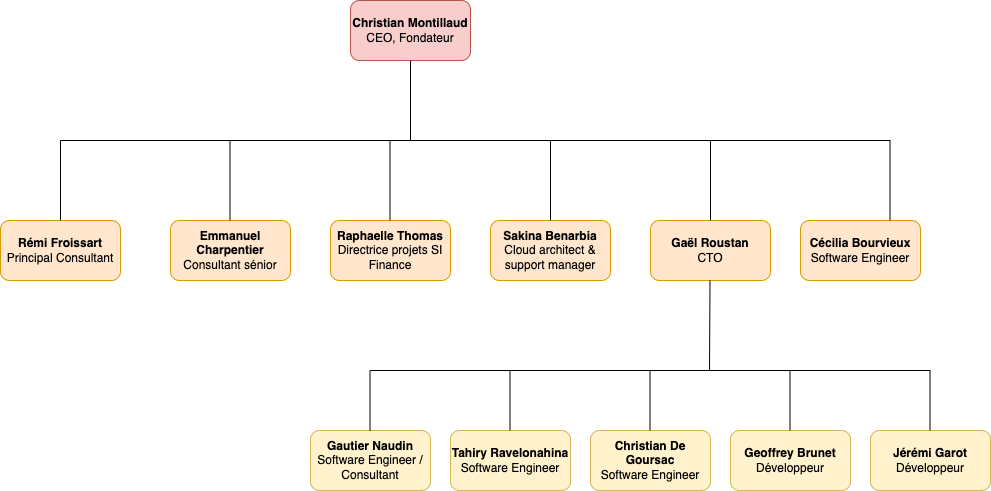
\includegraphics[scale=0.42,center]{schemas/organigramme-quartz-insight.png}
    \caption{Organigramme de Quartz-Insight}
\end{figure}
La société est gérée par monsieur Christian Montilaud.
Monsieur Gaël Roustan, est directeur technique et supervise le pôle Recherche et Développe\-ment.
Madame Cécilia Bourvieux gère un projet de test de charge pour les solutions de BI, du développement logiciel à la mise en place et l’exécution chez les clients.
Les membres du pôle R\&D (Recherche et développement) ont en charge le développement des Add-Ins pour les logiciels de chez Microsoft et Google, ainsi que la création, la mise en production et la gestion des microservices sous-jacents, avec l’aide de notre CTO.
Le reste des collaborateurs sont des consultants apportant leurs expertises dans leurs domaines respectifs chez nos différents clients.
\newline
\newline
Je suis donc actuellement développeur au sein du pôle R\&D, et travaille sur différents projets et microservices, dans le but d’améliorer ceux existants, résoudre des bugs et en créer de nouveaux lorsque cela est nécessaire.

\begin{figure}
  \section{Présentation de l'étudiant}
  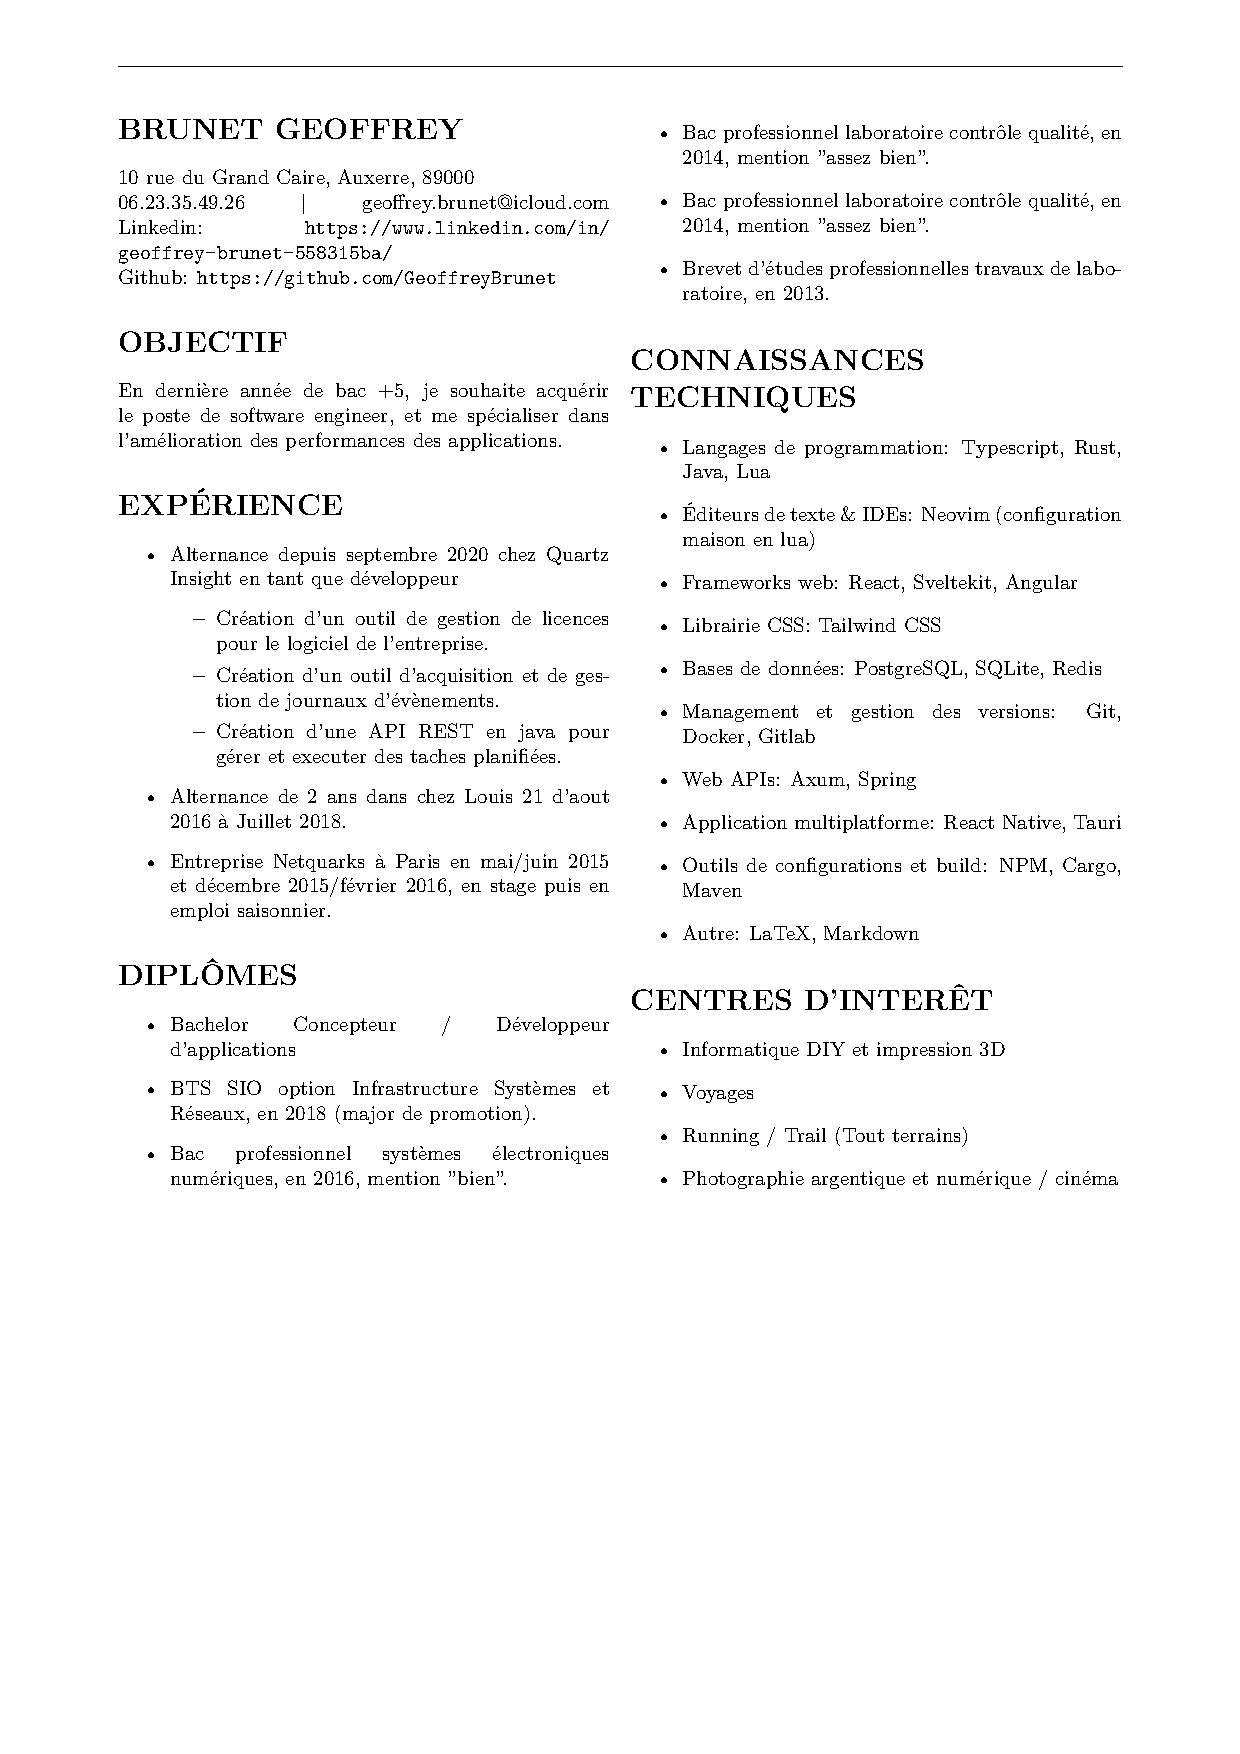
\includegraphics[scale=0.85, trim=2cm 0 0 0, clip]{CV-Geoffrey-Brunet.pdf}%
\end{figure}

\section{Activités de la structure}
Quartz-Insight est une entreprise spécialisée dans la Business Intelligence (BI) et l'Enterprise Performance Management (EPM).
Elle propose une gamme complète d'activités et de services destinés à aider les entreprises à optimiser leur gestion et à prendre des décisions éclairées. Voici un aperçu de nos principales activités:
\begin{enumerate}
  \item \textbf{Consulting en BI et EPM}: Quartz-Insight offre des services de consulting personnalisés pour accompagner les entreprises dans leur utilisation efficace des outils de BI et d'EPM tels que les serveurs Essbase, les cubes OLAP et Hyperion Planning.
    \ Les consultants de Quartz-Insight travaillent en étroite collaboration avec les clients pour comprendre leurs besoins spécifiques et proposer des solutions adaptées à leurs objectifs.
  \item \textbf{Réalisation de tests de charges sur des infrastructures de BI et d’EPM}: nous proposons une prestation de tests de charges pour les infrastructures BI et EPM des entreprises, avec divers scénarios possibles, pour tester les limites du matériel physique comme du logiciel.
    \ Le produit final est un fichier PDF contenant les résultats sous forme de graphs, ainsi qu’une proposition d’actions à mettre en place pour améliorer la résilience de l’infrastructure.
  \item \textbf{Développement de Qibates}: développement d’un logiciel en mode SAAS (Software As A Service) pour explorer diverses sources de bases de données multidimensionnelles.
    \ Un abonnement par licence par utilisateur est proposé à la vente, pour une utilisation sur Microsoft Excel ou Google Sheets, avec des accès à des sources de données diverse grâce à des connecteurs développés par nos soins. 
  \item \textbf{Conseil sur la transition RSE des entreprises}: après une implementation d’actions RSE (Responsabilité sociétale des entreprises) et de formations pour notre entreprise, nous avons décidé de proposer à nos clients une formation comprenant tous les principaux axes des actions mises en place.
    \ Nos proposons aussi une animation pour la fresque du climat, pour démontrer l’implication écologique pour les personnes comme pour les entreprises.
\end{enumerate}

\section{Présentation des activités confiées}
Voici une liste contenant les tâches qui m’ont été confiées durant mon alternance chez Quartz-Insight:
\begin{itemize}
  \item Écriture de fichiers « Dockerfile » pour la conteneurisation de nos microservices
  \item Résolution de tickets d’incidents sur l’add-in QiBates pour Google Sheets
  \item Écriture d’un logiciel de récupération de journaux d’évènements, avec une page web pour les consulter
  \item Collaboration pour développer une API REST sur un projet pour un de nos client (BNP)
  \item Transformation d’un ancien service monolithique en microservices pour la gestion des licences utilisateurs
\end{itemize}

\section{Présentation du Système d’Information}
Comme vu précédemment, le pôle Recherche et Développement édite des logiciels sous forme d’Add-In pour Google Sheets, Google Slides et Microsoft Excel, pour la manipulation de bases de données multidimensionnelles et d’outils de Planning.
Pour un soucis de performance, le traitement des données n’est pas fait sur le frontend de nos Add-Ins mais par des microservices hébergés sur nos machines virtuelles, dans un format de conteneur Docker.
\newline
\newline
Tous les microservices nécessitant d’être déployé sur des serveurs le seront sur des machines virtuelles hébergées chez notre partenaire OBS (pour Orange Business Services, filiale cloud du groupe Orange).
Ces machines virtuelles utilisent Docker pour gérer les cycles de vie des conteneurs.
Il en vas de même pour les bases de données, que nous utilisons en version managée, donc dont toute la partie serveur est gérée par OBS directement.

\chapter{Valorisation des compétences}

\section{Présentation globale du projet}
En tant qu'alternant, le projet qui m'a été confié consistait à effectuer une transformation majeure d'un service existant, passant d'une architecture $\emph{monolithique}^4$ à une architecture de $\emph{microservices}^5$.
Le service initial comprenait une web UI, une $\emph{API REST}^3$ et une base de données destinées à stocker les informations des utilisateurs, telles que leurs noms, domaines d'entreprise et types de profil.
L'architecture monolithique, qui reposait sur $\emph{ASP.NET}^8$ avec SQL Server comme $\emph{SGBD}^7$, présentait des limitations en termes de flexibilité et d'évolutivité.
L'objectif principal était donc de repenser cette infrastructure afin de permettre une évolutivité améliorée et des performances optimisées.
Pour atteindre cet objectif, nous avons adopté une approche basée sur les microservices.
Cela impliquait de diviser le service en plusieurs composants indépendants, chacun étant responsable d'une fonction spécifique.
Ainsi, nous avons pu obtenir une architecture plus flexible, où chaque microservice peut être géré et déployé de manière autonome.
Dans le cadre de cette transformation, nous avons choisi d'utiliser $\emph{Angular}^9$ pour la web UI, offrant ainsi une expérience utilisateur réactive et enrichissante.
Pour l'API REST, nous avons opté pour $\emph{Spring Boot}^{10}$, un $\emph{framework}^6$ Java réputé pour sa simplicité et sa robustesse.
De plus, nous avons migré la base de données vers $\emph{PostgreSQL}^{11}$, un système de gestion de base de données open source réputé pour ses performances et sa fiabilité.
Toutes ces technologies sont identiques pour le reste de nos microservices, nous permettant d’avoir une architecture uniformisée.

\section{Activité 1 - cartographie complète du système d'information existant}
\subsection{Compétence et son fondement}
\textbf{Bloc de compétences}: A1 – Analyse et définition de la stratégie des systèmes d’information
\newline
\textbf{Compétence choisie}: A1C4 – Cartographier un système d’information existant selon les 4 niveaux (métier, fonctionnel, applicatif et infrastructure) afin d’avoir une bonne connaissance de l’ensemble de ses composants
\newline
\textbf{Détails}: Cette compétence consiste à valider mon aptitude à réaliser une cartographie du S.I. précisant pour chaque couche les éléments suivants:
\begin{itemize}
  \item préciser dans le schéma les entités et les systèmes (en lien avec les Process Métier)
  \item préciser l’architecture applicative globale (les logiciels, les services et l’analyse des flux de données)
  \item présenter dans son schéma l’Infrastructure logique (VLAN, adresse.IP, filtrage et routage) infrastructure physique (équipements).
\end{itemize}
Elle consiste aussi à démontrer une utilisation appropriée d’un logiciel de cartographie:
\begin{itemize}
  \item démarrage du logiciel adéquat
  \item temps d’utilisation approprié (min 10 minutes)
  \item le résultat de la cartographie informatique correspond aux attendus d’une cartographie d’un SI demandé par un comité de direction
\end{itemize}
\subsection{Présentation et réalisation de l'activité}
Une étape pour cartographier le système d'information existant selon les 4 niveaux (métier, fonctionnel, applicatif et infrastructure) serait la réalisation d'une analyse approfondie de l'environnement existant. Voici la suite d’étapes réalisées pour atteindre cet objectif:
\subsubsection{Collecte des informations}
Ce monolithe n’a pas de documentation proprement associée, la principale source de connaissance est son code source, présent dans son repository sur Gitlab.
Pour analyser le service monolithique et étant programmé en .net, j’ai utilisé l’IDE fournis par Microsoft, Visual Studio.
Les informations importantes à regarder pendant l’analyse du code sont:
\begin{enumerate}
  \item Les endpoints de l’API REST
  \item Les classes qui servent de modèles
  \item Les requêtes effectuées par l’ORM vers le SGBD
  \item Les autres microservices qui communiquent avec le monolithe.
\end{enumerate}
La base de donnée utilisée par le monolithe a été utile pour observer les données sauvegardées dans les tables, et les jointures entre elles.
Étant donné qu’il s’agit de Microsoft SQL Server comme service de gestion de base de données, j’ai utilisé SSMS (SQL Server Management Studio) pour effectuer mes recherches.
Pour ce qui est des diagrammes et schémas, je les ai réalisé après analyse et sont présent dans ce dossier dans la sous-section « Analyse applicative ».
\subsubsection{Identification des composants métier}
Après consultation de l’équipe de développement, ce service monolithique n’est utilisé que par les dit-membres de cette équipe. La console n’est accéssible et utilisée que par eux.
L’objectif de ce service est de sauvegarder l’état des comptes et domaines clients qui utilisent la solution QiBates, ainsi que le type de profil pour les comptes (qui défini quelles options sont accessibles ou non).
Côté client, si il n’a jamais souscrit à une ou plusieurs licences QiBates, un domaine avec le nom de l’entreprise est créé. Le client envoie une liste des utilisateurs, avec entre autre leurs adresses mails professionnelles, et le type de profile demandé pour chaque compte.
Toutes ces informations sont enregistrées dans un fichier CSV qui est envoyé au monolithe, que celui-ci utiliseras pour créer et écrire les comptes avec les bonnes informations dans la base de données.
\subsubsection{Analyse fonctionnelle}
Pour l'analyse fonctionnelle, j'ai divisé celle-ci en 6 sous-analyses distinctes:
\begin{enumerate}
  \item \textbf{Identification des fonctionnalités, qui sont}:
    \begin{itemize}
      \item Création de profils utilisateur avec des informations telles que leur nom, domaine d'entreprise et type de profil, ainsi que sa durée de validité.
      \item Recherche d'utilisateurs par domaine d'entreprise.
      \item Mise à jour des informations du profil utilisateur.
      \item Gestion de la durée de vie des profils avec possibilité de renouvellement ultérieur.
      \item Suppresion d'un utilisateur, voir d'un domaine.
    \end{itemize}
  \item \textbf{Définition des cas d'utilisation}:
    \begin{itemize}
      \item Demande de création d'un nouvel utilisateur ou de plusieurs utilisateurs par un membre du pôle R&D, avec validation du directeur technique ou du CEO, demande effecutée par un directeur technique ou un contrôleur de gestion, en fonction de nos clients.
      \item Modification d'un profil utilisateur par un membre du pôle R&D, avec validation du directeur technique ou du CEO.
      \item Suppression d'un profil utilisateur par un membre du pôle R&D, avec validation du directeur technique ou du CEO.
      \item Renouvellement de la durée de vie d'un profil utilisateur.
      \end{itemize}
    \item \textbf{Modélisation des flux de travail}:
    Imaginons un premier cas d'utilisation qui serait "Demande de création, modification ou suppression d'un profil utilisateur":
    \begin{itemize}
      \item Un de nos client nous envoie une demande de création, modification ou suppression d'un profil utilisateur avec les informations nécessaires.
      \item Le CEO ou le CTO valide la dite demande.
      \item Les modifications sont transmises au pôle R&D, et un membre de celui-ci apporte les modifications sur l'interface web de l'application.
    \end{itemize}
    Dans le cadre d'un renouvellement de la durée de vie d'un profil utilisateur qui serviras en second cas d'utilisation:
    \begin{itemize}
      \item Un de nos client nous envoie une demande de création, modification ou suppression d'un profil utilisateur avec les informations nécessaires.
      \item Le CEO ou le CTO valide la dite demande.
      \item Les modifications sont transmises au pôle R&D, et un membre de celui-ci apporte les modifications sur l'interface web de l'application.
    \end{itemize}
  \item \textbf{Définition des entrées et sorties}:
    \begin{itemize}
      \item Pour les demandes de création, modification ou suppression d'un profil utilisateur, les entrées comprennent les informations nécessaires pour le profil utilisateur concerné.
      \item Pour la demande de renouvellement de la durée de vie d'un profil utilisateur, l'entrée est l'identification du profil utilisateur concerné.
      \item La sortie attendue est la validation ou le refus de la demande par le directeur technique ou le CEO. Si la demande est validée, la sortie finale est la création, modification ou suppresion d'un ou plusieurs comptes.
    \end{itemize}
\end{enumerate}
\subsubsection{Analyse applicative}
  \begin{figure}[h]
    \centering
    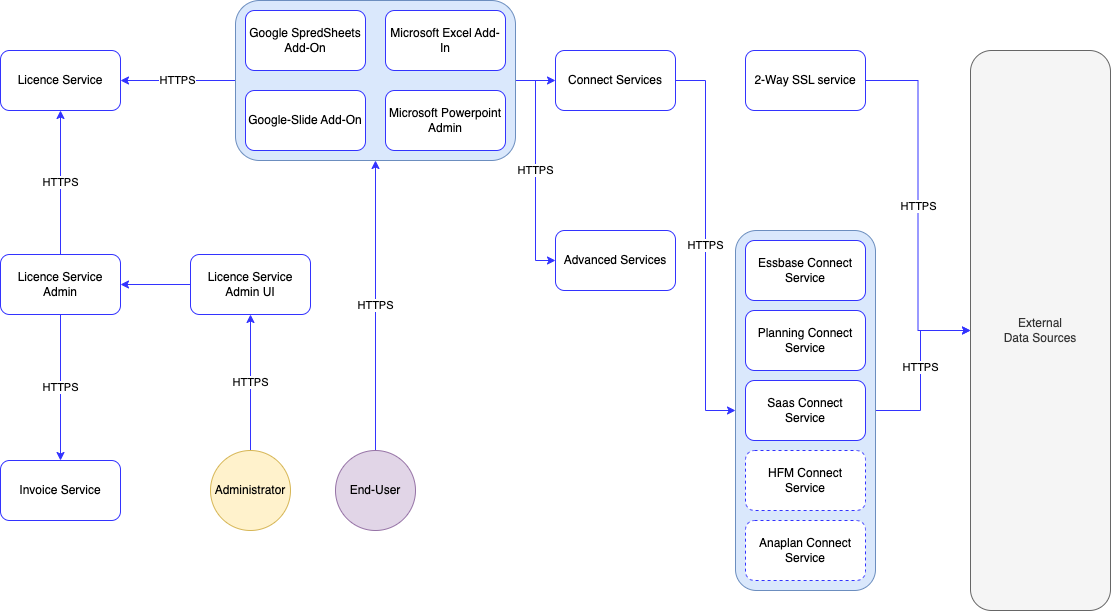
\includegraphics[scale=0.40,center]{schemas/schema-qibates-original.png}
    \caption{Schéma de l'infrastructure actuelle}
  \end{figure}
  Pour plus de clareté et de compréhension des rôles du service monolithique dans le schéma, celui-ci a été fragmenté, mais le monolithe contient tous les services du schéma suivants:
  \begin{itemize}
    \item \textbf{Licence service}: service qui permet de connaître l'existence d'un compte, son état et son profile.
    \item \textbf{Licence service Admin}: Partie backend permettant la création, modification et suppression des comptes, mais uniquement utilisable par un administrateur depuis l'interface web.
    \item \textbf{service Admin UI}: Interface web permettant la création, modification et suppression des comptes.
  \end{itemize}
  \begin{figure}[h]
    \centering
    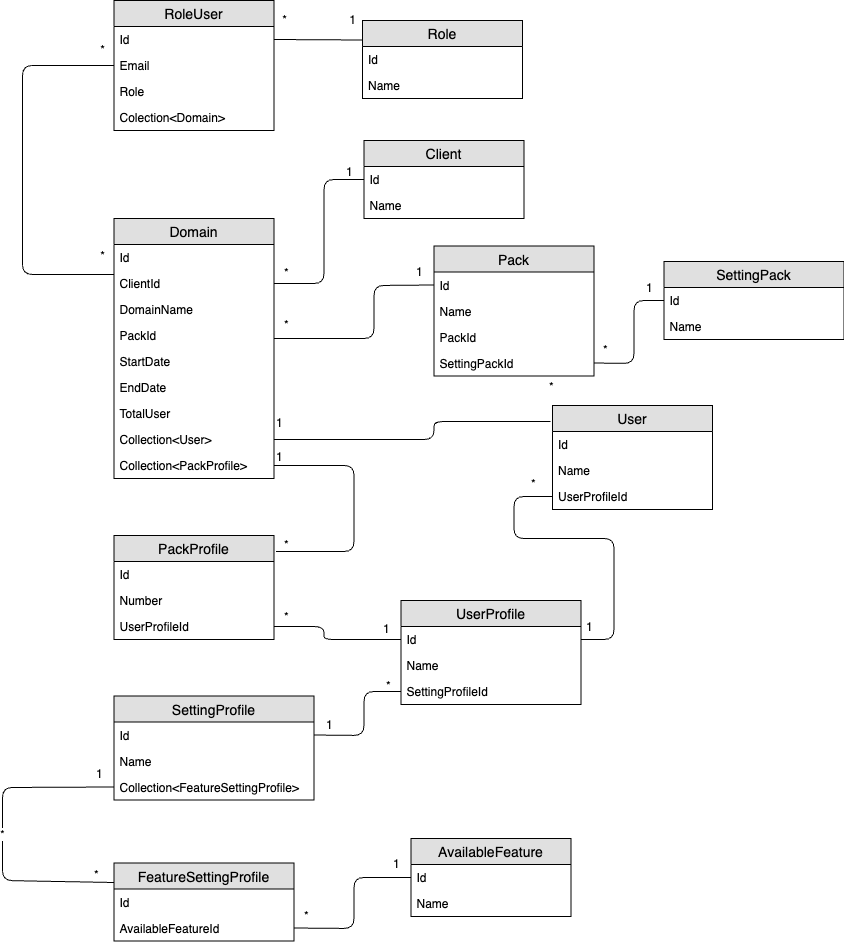
\includegraphics[scale=0.40,center]{schemas/ralph-diagram.png}
    \caption{Modèle de conception de données de la base de donnée du monolithe}
  \end{figure}
  Voici le MCD réalisé à partir des informations obtenues depuis le SGBD, et avec l'aide d'un collaborateur qui avais œuvré à son intégration.
  Une description de l'utilité de chaque table présente dans le schéma est effectuée ici:
  \begin{itemize}
    \item \textbf{Domain}: contient le domaine du client, ainsi que la durée de validité de ses comptes sous-jacents.
    \item \textbf{RoleUser}: utilisateur avec un rôle particulier pour l'administration de l'application.
    \item \textbf{Role}: role d'un utilisateur pour accéder et utiliser la console (droits de lecture ou rôle d'administrateur).
    \item \textbf{Client}: identifiant client, car un client peut avoir plusieurs domaines.
    \item \textbf{Pack}: permet de lier une liste prédéfinie de paramètres à un domaine (pour pouvoir les appliquer à tous les utilisateurs du domaine).
    \item \textbf{SettingPack}: liste prédéfinie de paramètres pour un utilisateur.
    \item \textbf{User}: utilisateur pour utiliser QiBates.
    \item \textbf{PackProfile}: permet de lier un domaine à un utilisateur.
    \item \textbf{UserProfile}: profile utilisateur permettant à un utilisateur d'avoir une liste de paramètres.
    \item \textbf{SettingProfile}: liste de paramètres de fonctionnalités pour un utilisateurs.
    \item \textbf{FeatureSettingProfile}: permet de changer les paramètres des fonctionnalités.
    \item \textbf{AvaibleFeature}: fonctionnalités spécifiques à QiBates (comme la coloration des cellules, le fait de se connecter à certains cubes, etc.).
  \end{itemize}

\subsubsection{Analyse de l'infrastructure}
Les exigences de l'infrascture sont définis sur 3 paramètres:
\begin{itemize}
  \item Performance: Le système doit être capable de traiter rapidement les demandes de création, modification ou suppression de profils, ainsi que les demandes de renouvellement.
  \item Sécurité: Les accès et les modifications aux profils utilisateurs doivent être contrôlés et sécurisés.
  \item Scalabilité: Le système doit être évolutif pour gérer une augmentation du nombre de demandes de gestion de profils sans compromettre les performances.
\end{itemize}
\newline
\newline
Chaque microservice est un conteneur Docker.
Nos serveurs Docker sont des machines virtuelles hébergées chez Orange Business Service, avec Ubuntu comme système d'exploitation.
Les caractéristiques physiques des machines virtuelles changent en fonction de la dite machine virtuelle, en fonction de l'OS (car nous avons aussi des machines virtuelles sur Windows pour les labs) et des zones de celle-ci (développement, pré-production et production).
\subsubsection{Documentation}
Toute l'analyse et la documentation produite a été mise à disposition des collaborateurs dans un dossier, sur le OneDrive (service de stockage en ligne collaboratif de chez Microsoft).
\subsection{Contexte de réalisation}
Cette activité a été réalisée en amon du projet, juste après la demande de refonte du service monolithique en microservices. Elle a donc été la première action réalisée après la dite demande.
\newline
\newline
Voici mes  éléments personnels quand à la réalisation de cette activitée :
\newline
J'ai utilisé mes compétences acquises en formation en architecture logicielle pour mieux analyser les différents microservices et leurs intéractions.
\newline
J'ai utilisé mes compétences en modélisation de données acquises au cours de ma formation pour la réalisation du MCD précédement présenté.
\newline
\newline
Ainsi que les éléments organisationnels et structurels :
\newline
J'ai analysé l'ancien SGBD pour comprendre comment les données étaient sauvegardées.
\newline
J'ai demandé aux autres dévelopeurs du pôle R&D quels microservices communiquent entre eux et comment pour réaliser le schéma précédent (numéro 4.1).
\subsection{Conclusion sur l'activité}
J'ai réalisé avec succès une cartographie complète du système d'information existant dans le cadre de la refonte du service monolithique en microservices.
J'ai utilisé mes compétences en architecture logicielle et en modélisation de données pour analyser les microservices et leurs interactions, les flux de données et les interactions entre les services.
Cette cartographie approfondie m'a permis d'identifier les fonctionnalités clés du projet, fournissant une base solide pour la conception des microservices.
J'ai mis à disposition de l'équipe la documentation complète pour faciliter la collaboration.
Mis à par un manque de documentation, aucun problème n'a eu lieu quand à la réalisation de cette activitée, donc les documents produits ont été validé par mon directeur technique.

\section{Activité 2 - cartographie des informations sensibles, évaluation des risques et définition d'une politique de sécurité}
\subsection{Compétence et son fondement}
\textbf{Bloc de compétences}: A1 – Analyse et définition de la stratégie des systèmes d’information
\newline
\textbf{Compétence choisie}: A1C5 – Identifier les informations sensibles, les risques, les zones critiques et les chemins d’attaque possibles d’un système d’information existant à l’aide de la cartographie afin d’aider le/la RSSI à définir une politique de sécurité
\textbf{Détails}: Cette compétence consiste à démontrer ma capacité à présenter une cartographie des risques du SI analysant les éléments suivants :
\begin{itemize}
  \item la confidentialité : préciser les règles d’authentification et d’accès aux ressources informatiques du SI
  \item l’intégrité : préciser les règles garantissant l’exactitude, la complétude et la non altération des données du SI;
  \item la disponibilité : préciser les procédures mises en place pour garantir la disponibilité des ressources informatiques du SI.
  \item formaliser à l’écrit une analyse du résultat de cette cartographie mettant en exergue les risques et zones critiques du SI
\end{itemize}
\subsection{Présentation et réalisation de l'activité}
  \subsubsection{Analyse de l'existant et des points chauds}
  Voici les informations principales relatives à la sécurité actuellement mise en place, en amont de la réalisation d'un PSSI (Politique de sécurité du système d'information):
  \begin{itemize}
    \item la confidentialité: Les accès aux ressources ce font avec des rôles définis par le directeur technique et en accord avec les membres du pôle R&D.
    La double authentification est obligatoire, ainsi qu'un mot de passe répondant à une politique définie au préalable.
    Les données dans les bases de données sont chiffrées.
    \item l’intégrité: préciser les règles garantissant l’exactitude, la complétude et la non altération des données du SI ;
    une sauvegarde incrémentale des bases de données a lieu chaque jour et les journaux d'événements sont aussi sauvegardés.
    \item la disponibilité: un démarrage d'un nouveau SGBD avec une sauvegarde de l'ancienne base de données peut être réalisé depuis OBS rapidement mais (mais aucun système de réplication comme avec PG-Pool II n'est actuellement en place).
  \end{itemize}
  \newline
  \newline
  Voici la liste des points chauds présents dans la réalisation de ce projet:
  \begin{enumerate}
    \item \textbf{La migration de la base de données} peut être un point chaud en raison du risque de perte de données ou de corruption pendant le processus de migration.
    \item \textbf{La sécurité des microservices}, la communication entre les microservices, l'authentification des utilisateurs et la gestion des autorisations  sont des points critiques qui doivent être soigneusement mis en place pour éviter les vulnérabilités potentielles.
    \item \textbf{La gestion des accès aux API}, avec la gestion des identifiants et des jetons d'authentification doit être sécurisée pour protéger les ressources sensibles.
    \item \textbf{La sécurité de l'interface web}, dont celle-ci doit être protégée contre les attaques de sécurité courantes, telles que les attaques XSS (Cross-Site Scripting) ou les attaques CSRF (Cross-Site Request Forgery).
    \item \textbf{La gestion des privilèges d'accès} est cruciale pour éviter les fuites d'informations sensibles ou les accès non autorisés.
    \item \textbf{La surveillance et détection des incidents} pour détecter les activités anormales ou les tentatives d'intrusion est essentielle pour identifier rapidement les incidents de sécurité et y répondre de manière appropriée.
  \end{enumerate}
  Pour faciliter l'identification des informations sensibles, les risques, les zones critiques et les chemins d’attaque possibles, j'ai réalisé une première mouture d'un Plan de Sécurité des Systèmes d'Information (PSSI).
  Celui ci ce base sur 3 principaux axes, les principes organisationnels, les principes de mise en œuvre et les principes techniques.
  \subsubsection{}
  Voici les \textbf{principes organisationnels en œuvre} du projet de refonte du service:
  \begin{enumerate}
    \item \textbf{Politique de sécurité}:
      \begin{itemize}
        \item Élaboration d'une politique de sécurité qui définit les objectifs, les responsabilités et les exigences pour la sécurité de l'ensemble de l'organisation.
      \end{itemize}
    \item \textbf{Organisation de la sécurité}:
      \begin{itemize}
        \item Établissement d'une structure des organisations claire pour la gestion de la sécurité, avec une identification des responsabilités et des rôles spécifiques liés à la sécurité de l'information.
        \item Désignation d'un RSSI (Responsable de la sécurité des systèmes d'information) chargé de coordonner les activités de sécurité et de veiller à leur mise en œuvre.
      \end{itemize}
    \item \textbf{Gestion des risques SSI}:
      \begin{itemize}
        \item Mise en place un processus de gestion des risques pour identifier, évaluer et traiter les risques liés à la sécurité de l'information.
        \item Développement des plans d'action pour atténuer les risques identifiés.
      \end{itemize}
    \item \textbf{Sécurité et cycle de vie}:
      \begin{itemize}
        \item Intégration des principes de sécurité dès les phases de conception, de développement, de déploiement et de maintenance du système.
        \item Mise en place d'évaluations régulières de sécurité tout au long du cycle de vie du projet pour identifier les vulnérabilités et prendre les mesures correctives nécessaires.
      \end{itemize}
    \item \textbf{Assurance et certification}:
      \begin{itemize}
        \item Établissement des mécanismes d'assurance et de certification pour valider la conformité de votre système à des  normes et réglementations en matière de sécurité.
        \item Recherche des certifications appropriées, telles que ISO 27001 (norme relative à la sécurité), pour attester de la maturité et de la conformité de votre système en matière de sécurité.
      \end{itemize}
  \end{enumerate}
  \subsubsection{}
  Voici les \textbf{principes de mise en œuvre} du projet de refonte du service:
  \begin{enumerate}
    \item \textbf{Aspects humains}:
      \begin{itemize}
        \item Implication les parties prenantes clés, telles que le directeur technique, le CEO, les membres du pôle R&D, et confirmer leurs engagements envers les objectifs de sécurité du projet, au travers de réunions.
        \item Établissement clair des rôles et des responsabilités en matière de sécurité, en définissant les tâches et les autorisations appropriées pour chaque acteur du projet (en corrélation avec les différents droits d'administration du service gestionnaire de licences).
      \end{itemize}
    \item \textbf{Planification de la continuité des activités}:
      \begin{itemize}
        \item Identification des activités critiques du système et élaboration de plans de continuité des activités pour assurer leur disponibilité en cas d'incident ou de sinistre.
        \item Mise en place de mécanismes de sauvegarde réguliers et des procédures de récupération des données pour minimiser les temps d'arrêt et préserver l'intégrité des informations.
      \end{itemize}
    \item \textbf{Gestion des incidents}:
      \begin{itemize}
        \item Création et écriture de procédures claires pour la gestion des incidents de sécurité, y compris la notification, l'investigation, la résolution et le suivi.
        \item Mise en place d'une ou plusieurs personnes pour répondre rapidement aux incidents et atténuer les impacts.
      \end{itemize}
    \item \textbf{Sensibilisation et formation}:
      \begin{itemize}
        \item Mise en place de sessions de sensibilisation à la sécurité pour les employés (clients comme internes à Quartz Insight), afin de les informer des meilleures pratiques, des politiques et des procédures de sécurité. \
          Cela peux faire référence à des points comme le SSO, la double authentification, la gestion des mots de passe le fait de vérouiller son poste lorsqu'un utilisateur utilise QiBates et s'absente de son poste).
      \end{itemize}
    \item \textbf{Exploitation}:
      \begin{itemize}
        \item Mise en place d'une solution de supervision en temps réel, avec une définition des métriques et journaux d’évènements, au préalable.
        \item Formation des membres du pôle R&D à la lecture et l'analyse des dites métriques et des dits journaux d’évènements.
        \item Écriture d'une politique de mise à jour des micro-services pour réduire le temps d'arrêt à un strict minimum.
      \end{itemize}
    \item \textbf{Aspects physiques et environnementaux}:
      \begin{itemize}
        \item Mise à part les ordinateurs portables, Quartz-Insight ne possède aucune machine physique.
        \item Nos machines virtuelles sont toutes hébergées chez Orange Business Service (OBS), dans des régions.
        \item Un accès VPN est requis pour accéder aux serveurs et applications en cours de dévellopement, en plus d'un couple identifiant et mot de passe propre à chacun.
      \end{itemize}
  \end{enumerate}
  \subsubsection{PSSI}
  Voici une analyse des \textbf{principes techniques} de la PSSI:
  \begin{enumerate}
    \item \textbf{Identification des composants métier}:
      \begin{itemize}
        \item Le système comprendra les composants métier suivants : interface web, API REST et base de données.
        \item L'interface web sera développée en utilisant Angular.
        \item L'API REST sera développée avec Spring Boot.
        \item La base de données sera migrée vers PostgreSQL, un système de gestion de base de données open source réputé pour ses performances et sa fiabilité.
        \item Les autres microservices du projet utiliseront également ces technologies pour uniformiser l'architecture.
      \end{itemize}
    \item \textbf{Gestion des accès et des privilèges}:
      \begin{itemize}
        \item Les utilisateurs doivent s'authentifier avant d'accéder au système, en utilisant des identifiants et des mots de passe, ainsi qu'un compte Google ou Microsoft pour le SSO.
        \item Des politiques de contrôle des privilèges sont mises en place pour limiter l'accès aux fonctionnalités et aux données sensibles.
        \item Les membres du pôle R&D auront des privilèges spécifiques pour créer, modifier et supprimer des profils utilisateurs, sous réserve de validation par le directeur technique ou le CEO.
      \end{itemize}
    \item \textbf{Protection des données}:
      \begin{itemize}
        \item Les données des utilisateurs, telles que leurs noms, domaines d'entreprise et types de profil, seront stockées dans la base de données PostgreSQL.
        \item Des mesures de sécurité, telles que le chiffrement des données sensibles et la sauvegarde régulière des données, seront mises en place pour assurer la confidentialité et la disponibilité des données.
        \item Un cluster de SGBD peut être mis en place, avec un outil logiciel comme PG-Pool II.
      \end{itemize}
    \item \textbf{Surveillance et détection des incidents}:
      \begin{itemize}
        \item Un système de surveillance des activités anormales et des incidents de sécurité est mis en place pour détecter les éventuelles violations de sécurité ou les comportements suspects. \
          Il utilise notre système de supervision et de gesiton de journaux d'évènements.
        \item Des procédures de gestion des incidents seront définies, notamment pour la notification, l'investigation, la résolution et le suivi des incidents de sécurité.
      \end{itemize}
    \item \textbf{Conformité et réglementations}:
      \begin{itemize}
        \item Le projet doit se conformer aux réglementations applicables en matière de protection des données et de confidentialité, telles que le RGPD (Règlement général sur la protection des données).
        \item Des audits réguliers seront effectués pour évaluer la conformité et l'efficacité des mesures de sécurité mises en place.
      \end{itemize}
  \end{enumerate}
  Les 4 critères de sécurité pour le service d'information (SI) dans un PSSI sont:
  \begin{enumerate}
    \item \textbf{Confidentialité}: le SI de mettre en place une politique de gestion des droits pour avoir la fiabilité que seules les personnes autorisées ont accès aux données.
    \item \textbf{Disponibilité}: le SI doit rendre accessible les données, rapidement et avec une constance dans le temps.
    \item \textbf{Intégrité}: le SI doit être en mesure de vérifier et prouver qu'aucune modification n'a été apportée aux données.
    \item \textbf{Tracabilité}: le SI doit mettre en place un historique des accès aux données, historique qui se doit d'être lisible et vérifiable.
  \end{enumerate}
  \subsubsection{Norme ISO 27000}
  Comme indiqué précédement dans le PSSI, être conforme à la norme ISO 27000 serais un avantage considérable, car elle est un ensemble de normes internationales qui fournit des lignes directrices et des bonnes pratiques pour la gestion de la sécurité de l'information au sein d'une organisation.
  Voici les principales recommendations après une lecture des documents des normes ISO 27000, 27001, 27005, et une liste de d'actions à mettre en place pour y répondre:
  \begin{enumerate}
    \item \textbf{Politique de sécurité}: élaboration d'une politique de sécurité claire et documentée qui énonce les principes, les objectifs et les responsabilités en matière de sécurité de l'information.
    \item \textbf{Gestion des risques}: effectuer une évaluation approfondie des risques liés à la totalité des microservices de QiBates, en identifiant les informations sensibles, les menaces potentielles et les vulnérabilités.
      \ Établissement de mesures de sécurité appropriées pour atténuer ces risques.
    \item \textbf{Contrôles de sécurité}: mise en place des contrôles de sécurité techniques et managériales conformes aux recommandations de la norme ISO 27000.
      \ cela peut inclure la mise en œuvre de mécanismes d'authentification (0Auth a été utilisé pour ce projet) et d'autorisation, le chiffrement des données, la surveillance des activités, la gestion des journaux (avec Loki et Grafana) et la protection contre les attaques.
    \item \textbf{Sensibilisation et formation}: sensibilisation et formation des membres de l'équipe du le projet aux principes de sécurité de l'information, aux bonnes pratiques de développement sécurisé et aux politiques de sécurité établies.
    \item \textbf{Gestion des incidents}: mise en place un processus de gestion des incidents pour détecter, signaler, investiguer et répondre aux incidents de sécurité éventuels.
      \ Établissement de mécanismes de signalement des incidents et vérification de l'application des mesures correctives appropriées.
    \item \textbf{Évaluation et amélioration continue}: effectuer des audits réguliers pour évaluer la conformité aux exigences de la norme ISO 27000 et pour identifier les domaines d'amélioration.
      \ Mise en place un processus d'amélioration continue pour renforcer la sécurité de l'information tout au long du projet.
  \end{enumerate}
  \subsection{Contexte de réalisation}
La mise en place du PSSI et de l'analyse des normes ISO a été réalisée en cours de projet, après le prototypage de celui-ci, mais avant la mise en production des micro-services développés.
\newline
\newline
Voici mes éléments personnels quand à la réalisation de cette activitée:
\newline
Grâce à notre formation en RGPD et sécurité des S.I. suivie en entreprise, j'ai été informé des principes de protection des données et des bonnes pratiques de sécurité.
\newline
La formation sur les normes ISO 27000 et sur la réalisation d'un PSSI, suivie à l'EPSI, m'a doté d'une solide compréhension des normes de sécurité de l'information et des étapes nécessaires pour mettre en place un PSSI.
\newline
\newline
Ainsi que les éléments organisationnels et structurels :
\newline
En me référant à différents PSSI trouvés en ligne, j'ai lu et analysé les bonnes pratiques de sécurité de l'information mises en œuvre par d'autres organisations pour les adapter à mon projet (tel le PSSI de l'université de Poitiers).
\newline
Le formateur de l'EPSI m'a fourni des ressources telles que les normes ISO 27000-27001-27002-27005, me permettant de me familiariser avec les exigences et les recommandations des normes citées précédement.
\subsection{Conclusion sur l'activité}
J'ai donc realisé une maquête de PSSI et une analyse des normes ISO 27000 dans le cadre de cet activité. La formation à l'EPSI ainsi que l'application pour ce projet m'a permis de capitaliser et d'appliquer mes connaissances dans une situation concrête.
\newline
Les analyses produites m'ont servis pendant la réalisaiton du projet, pour analyser les points sensibles des microservices, et d'actions à mettre en place pour améliorer la sécurité du système d’information.
\newline
\newline
Les évolutions possibles sont les mises à jour des normes ISO, et des bonnes pratiques pour la réalisation d'un PSSI, tout en effectuant une veille sur la sécurité informatique.

\section{Activité 3 - analyse des données de références pour la création d'un référentiel de données}
\subsection{Compétence et son fondement}
\textbf{Bloc de compétences}: A4 – Pilotage de l’informatique décisionnelle d’un système d’information (business intelligence & big data)
\newline
\textbf{Compétence choisie}: A4C6 – Définir les données de référence de l’entreprise à partir des données utilisées pour créer un référentiel de données afin d’assurer la mise à disposition de données cohérentes aux directions métiers
\newline
\textbf{Détails}: Cette compétence consiste à démontrer ma capacité à identifier le référentiel de donnée de l’entreprise :
\begin{itemize}
  \item identifier et formalisre par écrit des critères de sélection et de validation des données existantes.
\end{itemize}
\subsection{Présentation et réalisation de l'activité}
  Dans le chapitre "4.2.2", avec la figure "4.2 - Modèle de conception de données de la base de donnée du monolithe" et la description présente en dessous, le MCD est présent avec la description de chaque table.
  L'architecture microservices m'a orienté quand à la division de la précédente base de données en 3 nouvelles bases de données distinctes.
  \newline
  Voici en dessous chaque MCD pour chacune des 3 bases de données, ainsi que la description de celui-ci.
  Voici la description de la base de données pour sauvegarder les fonctionnalités:
  \begin{itemize}
    \item \textbf{Domain}: enregistre le domaine du client.
    \item \textbf{User}: enregistre le nom de l'utilisateur.
    \item \textbf{FeatureGroup}: enregistre un groupe de fonctionnalités.
    \item \textbf{Feature}: enregistre une fonctionnalité.
  \end{itemize}
  \begin{figure}[H]
      \centering
      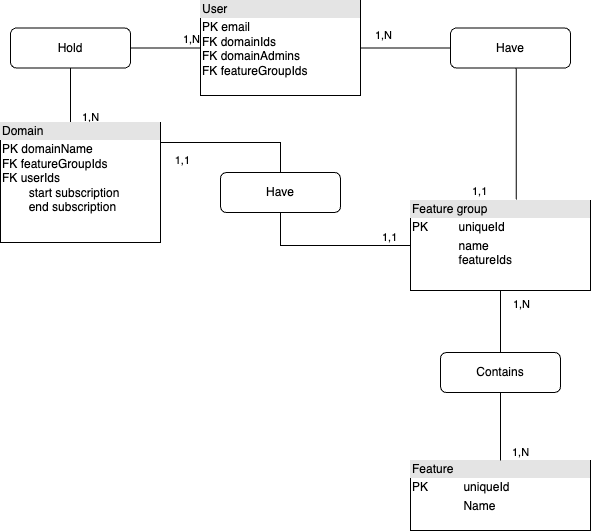
\includegraphics[scale=0.40,center]{schemas/features-mcd-ralph2.png}
      \caption{Modèle de conception de données des domaines clients}
  \end{figure}
  Voici la description de la base de données pour sauvegarder les paramètres des utilisateurs:
  \begin{itemize}
    \item \textbf{Domain}: enregistre le domaine du client.
    \item \textbf{User}: enregistre le nom de l'utilisateur.
    \item \textbf{DomainUserSetting}: enregistre un groupe de paramètres pour l'utilisateur.
    \item \textbf{DefaultSetting}: enregistre un paramètre par défaut.
  \end{itemize}
  \begin{figure}[H]
      \centering
      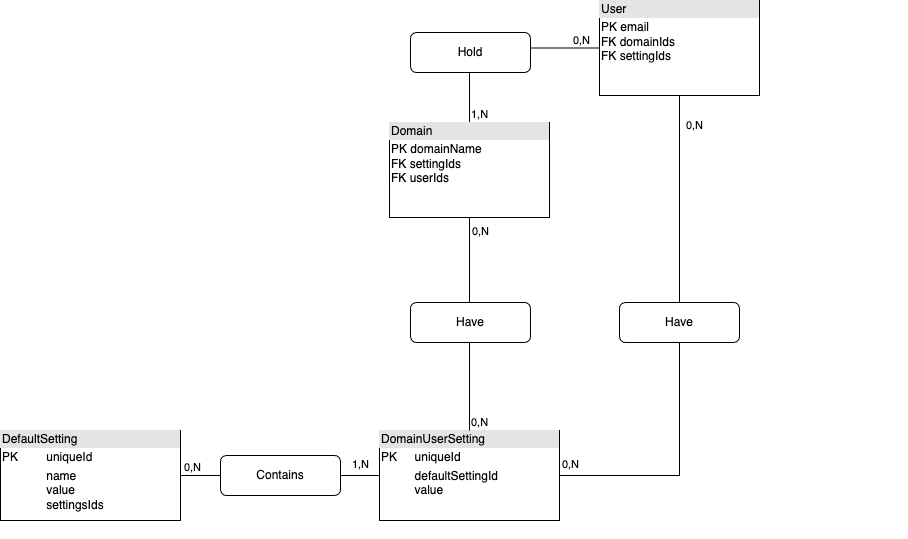
\includegraphics[scale=0.40,center]{schemas/settings-mcd-kingcandy.png}
      \caption{Modèle de conception de données pour la sauvegarde des paramètres clients}
  \end{figure}
  Voici la description de la base de données pour sauvegarder les notifications à envoyer:
  \begin{itemize}
    \item \textbf{Domain}: enregistre le domaine du client.
    \item \textbf{User}: enregistre le nom de l'utilisateur.
    \item \textbf{Notification}: enregistre les notifications à envoyer à l'utilisateur.
  \end{itemize}
  \begin{figure}[H]
      \centering
      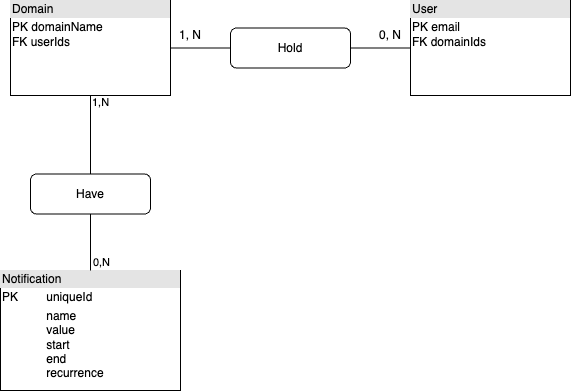
\includegraphics[scale=0.40,center]{schemas/notifications-mcd-calhoun.png}
      \caption{Modèle de conception de données de sauvegarde des notifications}
  \end{figure}
  Pour le choix du gestionnaire de base de données, j'ai utilisé le théorème CAP.
  Il permet selon 3 critères, de séléctionner un SGBD en fonction des problématiques auquelles il doit répondre, comme la disponibilité, la cohérence et la distributivité.
  La volonté de garder un SGBD avec un modèle relationnel, et en prenant en compte les autres SGBD présents dans l'infrastructure de QiBates, le choix c'est porté sur PostgreSQL, étant Open Source, et ayant une bonne documentation ainsi qu'une grande communauté.
  \begin{figure}[H]
      \centering
      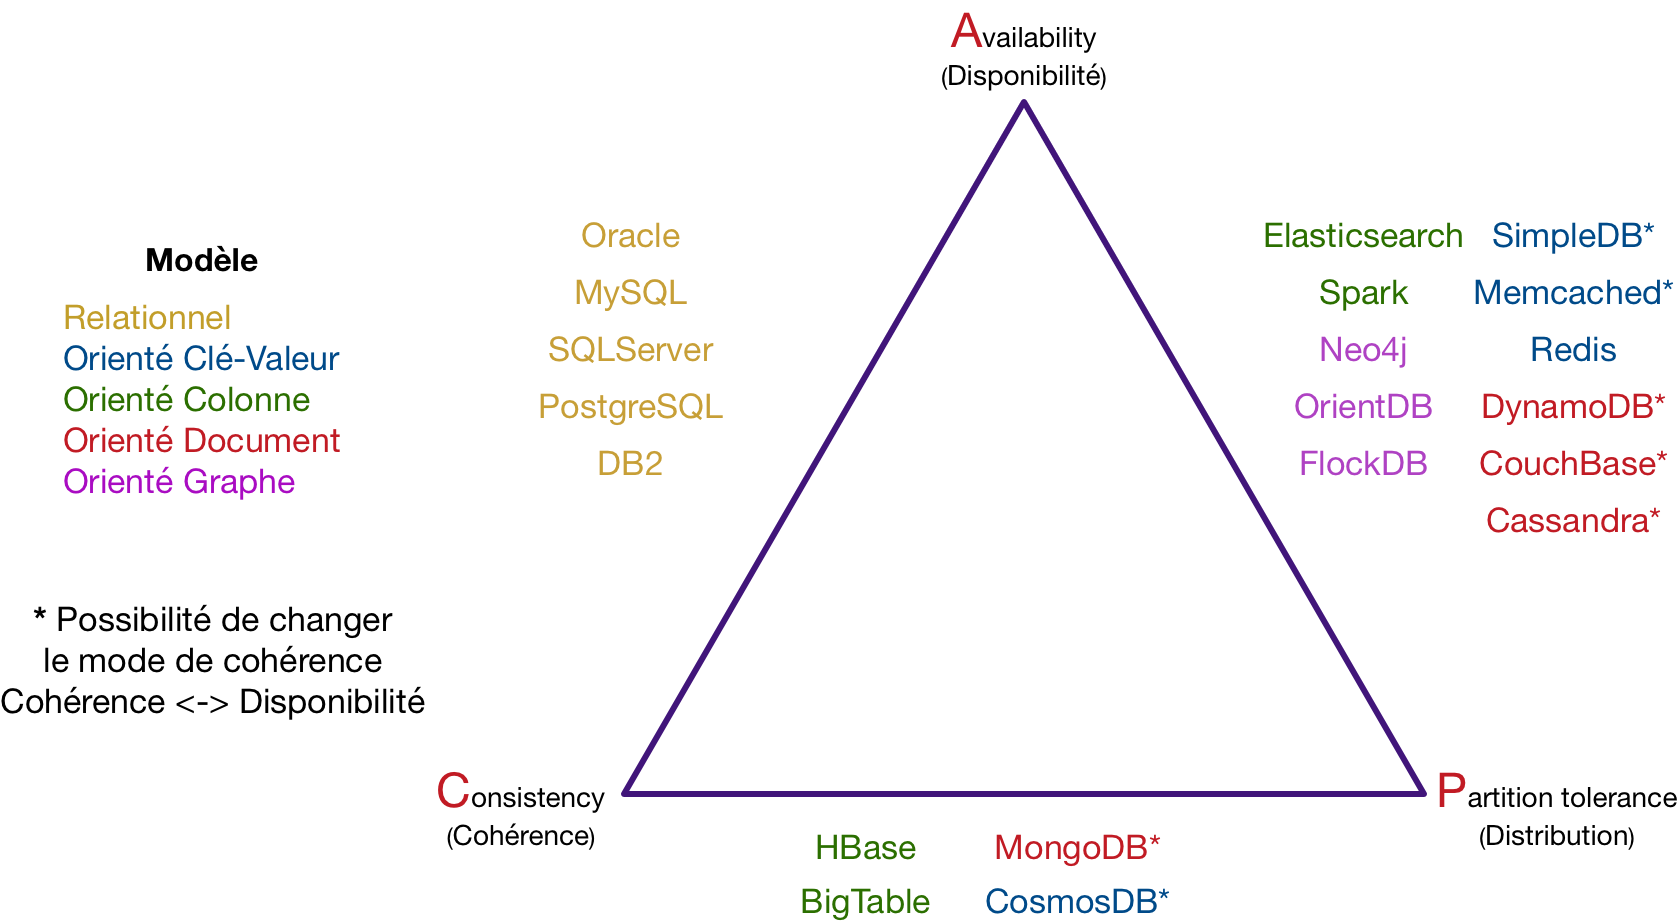
\includegraphics[scale=0.25,center]{schemas/cap-theoreme.png}
      \caption{Théorème CAP}
  \end{figure}
  \newline
  Chacune des 3 bases de données seras présente sur le même SGBD pour des raisons de coûts et de maintenance, car permettant d'éviter de payer 3 SGBD chez OBS, et n'ayant qu'un seul SGBD à répliquer, avec un outil comme PG-Pool II.
\subsection{Contexte de réalisation}
J'ai collaboré avec un développeur pour valider les MCD, et obtenu l'approbation de mon directeur technique après lui avoir présenté la refonte totale du SGDB.
Trois bases de données ont ainsi été créées pour stocker les fonctionnalités, les paramètres des utilisateurs et les notifications, avec PostgreSQL comme choix de gestionnaire de base de données, validé en considération de l'infrastructure existante.
Le SGBD est toujours managé par OBS, j'ai donc créé une nouvelle instance pour héberger les 3 nouvelles bases de données.

\subsection{Conclusion sur l'activité}
Au cours de cette activité, j'ai  exploré les tenants et aboutissants de l'analyse des données de référence pour la création d'un référentiel cohérent.
En adaptant le modèle conceptuel de données du monolithe à l'architecture microservices, j'ai orchestré la création de trois bases distinctes pour sauvegarder les fonctionnalités, les paramètres des utilisateurs et les notifications.
En optant pour PostgreSQL comme gestionnaire de base de données, en accord avec les besoins et la structure existante, j'ai mis en oeuvre mes capacités à réaliser cette activité, avec des choix justifiés et justifiables.
\newline
\newline
Pour les évolutions dans 10 ans, les bases de données relationnelles ainsi que les schémas sous-jacents comme les MCD seront toujours d'actualité pour la sauvegarde de données, malgré l'essort des SGBD NoSQL (Not Only SQL, sauvegardant des données en format clef-valeur, JSON ou autre).

\section{Activité 4 - analyse des besoins métiers pour une solution applicative sur mesure}
\subsection{Compétence et son fondement}
\textbf{Bloc de compétences}: A5 – Développement d’une solution applicative spécifique et métier selon le projet de développement S.I.
\newline
\textbf{Compétence choisie}: A5C1 – Collecter les besoins métiers des utilisateurs en menant des interviews auprès d’eux pour comprendre leurs activités et leurs contraintes métier afin d’étudier les opportunités et la faisabilité technologique d’une solution applicative spécifique ou métier
\newline
\textbf{Détails}: Cette compétence consiste à démontrer ma capacité à présenter mes éléments de préparation à la collecte des besoins en détaillant :
\begin{itemize}
  \item l’interview-type à mener avec le questionnaire à utiliser en précisant la méthodologie de retranscription (tableau, graphique,...)
  \item besoins métiers attendus par le client en termes de fonctionnalités
  \item contraintes métiers à prendre en compte
\end{itemize}
\subsection{Présentation et réalisation de l'activité}
\subsubsection{Étapes de réalisation de l'interview}
\begin{enumerate}
  \item Préparation de l'Interview :
  \begin{itemize}
    \item J'ai identifié les modules du monolithe à transformer en microservices.
    \item J'ai identifié les personnes clefs à interroger (trois développeurs du pôle R\&D seront intérrogés).
    \item J'ai créé un modèle d'interview incluant des questions sur les fonctionnalités actuelles, les défis rencontrés et les besoins non satisfaits.
  \end{itemize}
   \item Conduite des Interviews :
  \begin{itemize}
    \item J'ai réalisé une enquête avec Google forms
  \end{itemize}
  \item Identification des Besoins Métiers :
  \begin{itemize}
    \item J'ai analysé les réponses du formulaire pour identifier les besoins spécifiques.
    \item J'ai identifié les fonctionnalités clés à découper en microservices et les interactions nécessaires.
  \end{itemize}
  \item Formalisation des Contraintes Métiers :
  \begin{itemize}
    \item J'ai inclus les exigences de sécurité, de performances, d'évolutivité, etc.
  \end{itemize}
  \item Création des Questionnaires de Retranscription :
  \begin{itemize}
    \item J'ai créé des questionnaires spécifiques pour retranscrire les réponses des entretiens.
    \item J'ai utilisé des tableaux ou des graphiques pour organiser les besoins et contraintes.
  \end{itemize}
  \item Présentation des Résultats :
  \begin{itemize}
    \item J'ai présenté les besoins et contraintes identifiés pour chaque module aux parties prenantes.
    \item J'ai expliqué comment la transformation en microservices répondra aux besoins et contraintes métiers.
  \end{itemize}
\end{enumerate}
\subsubsection{Outil pour la réalisation de l'interview}
J'ai utilisé Google Forms, un outil de création de formulaire gratuit et en ligne, pour réaliser mon enquête.
Celui-ci m'a permis de présenter les questions et d'obtenir les réponses des personnes concernées directement sur la page associée au formulaire.
  \begin{figure}[H]
      \centering
      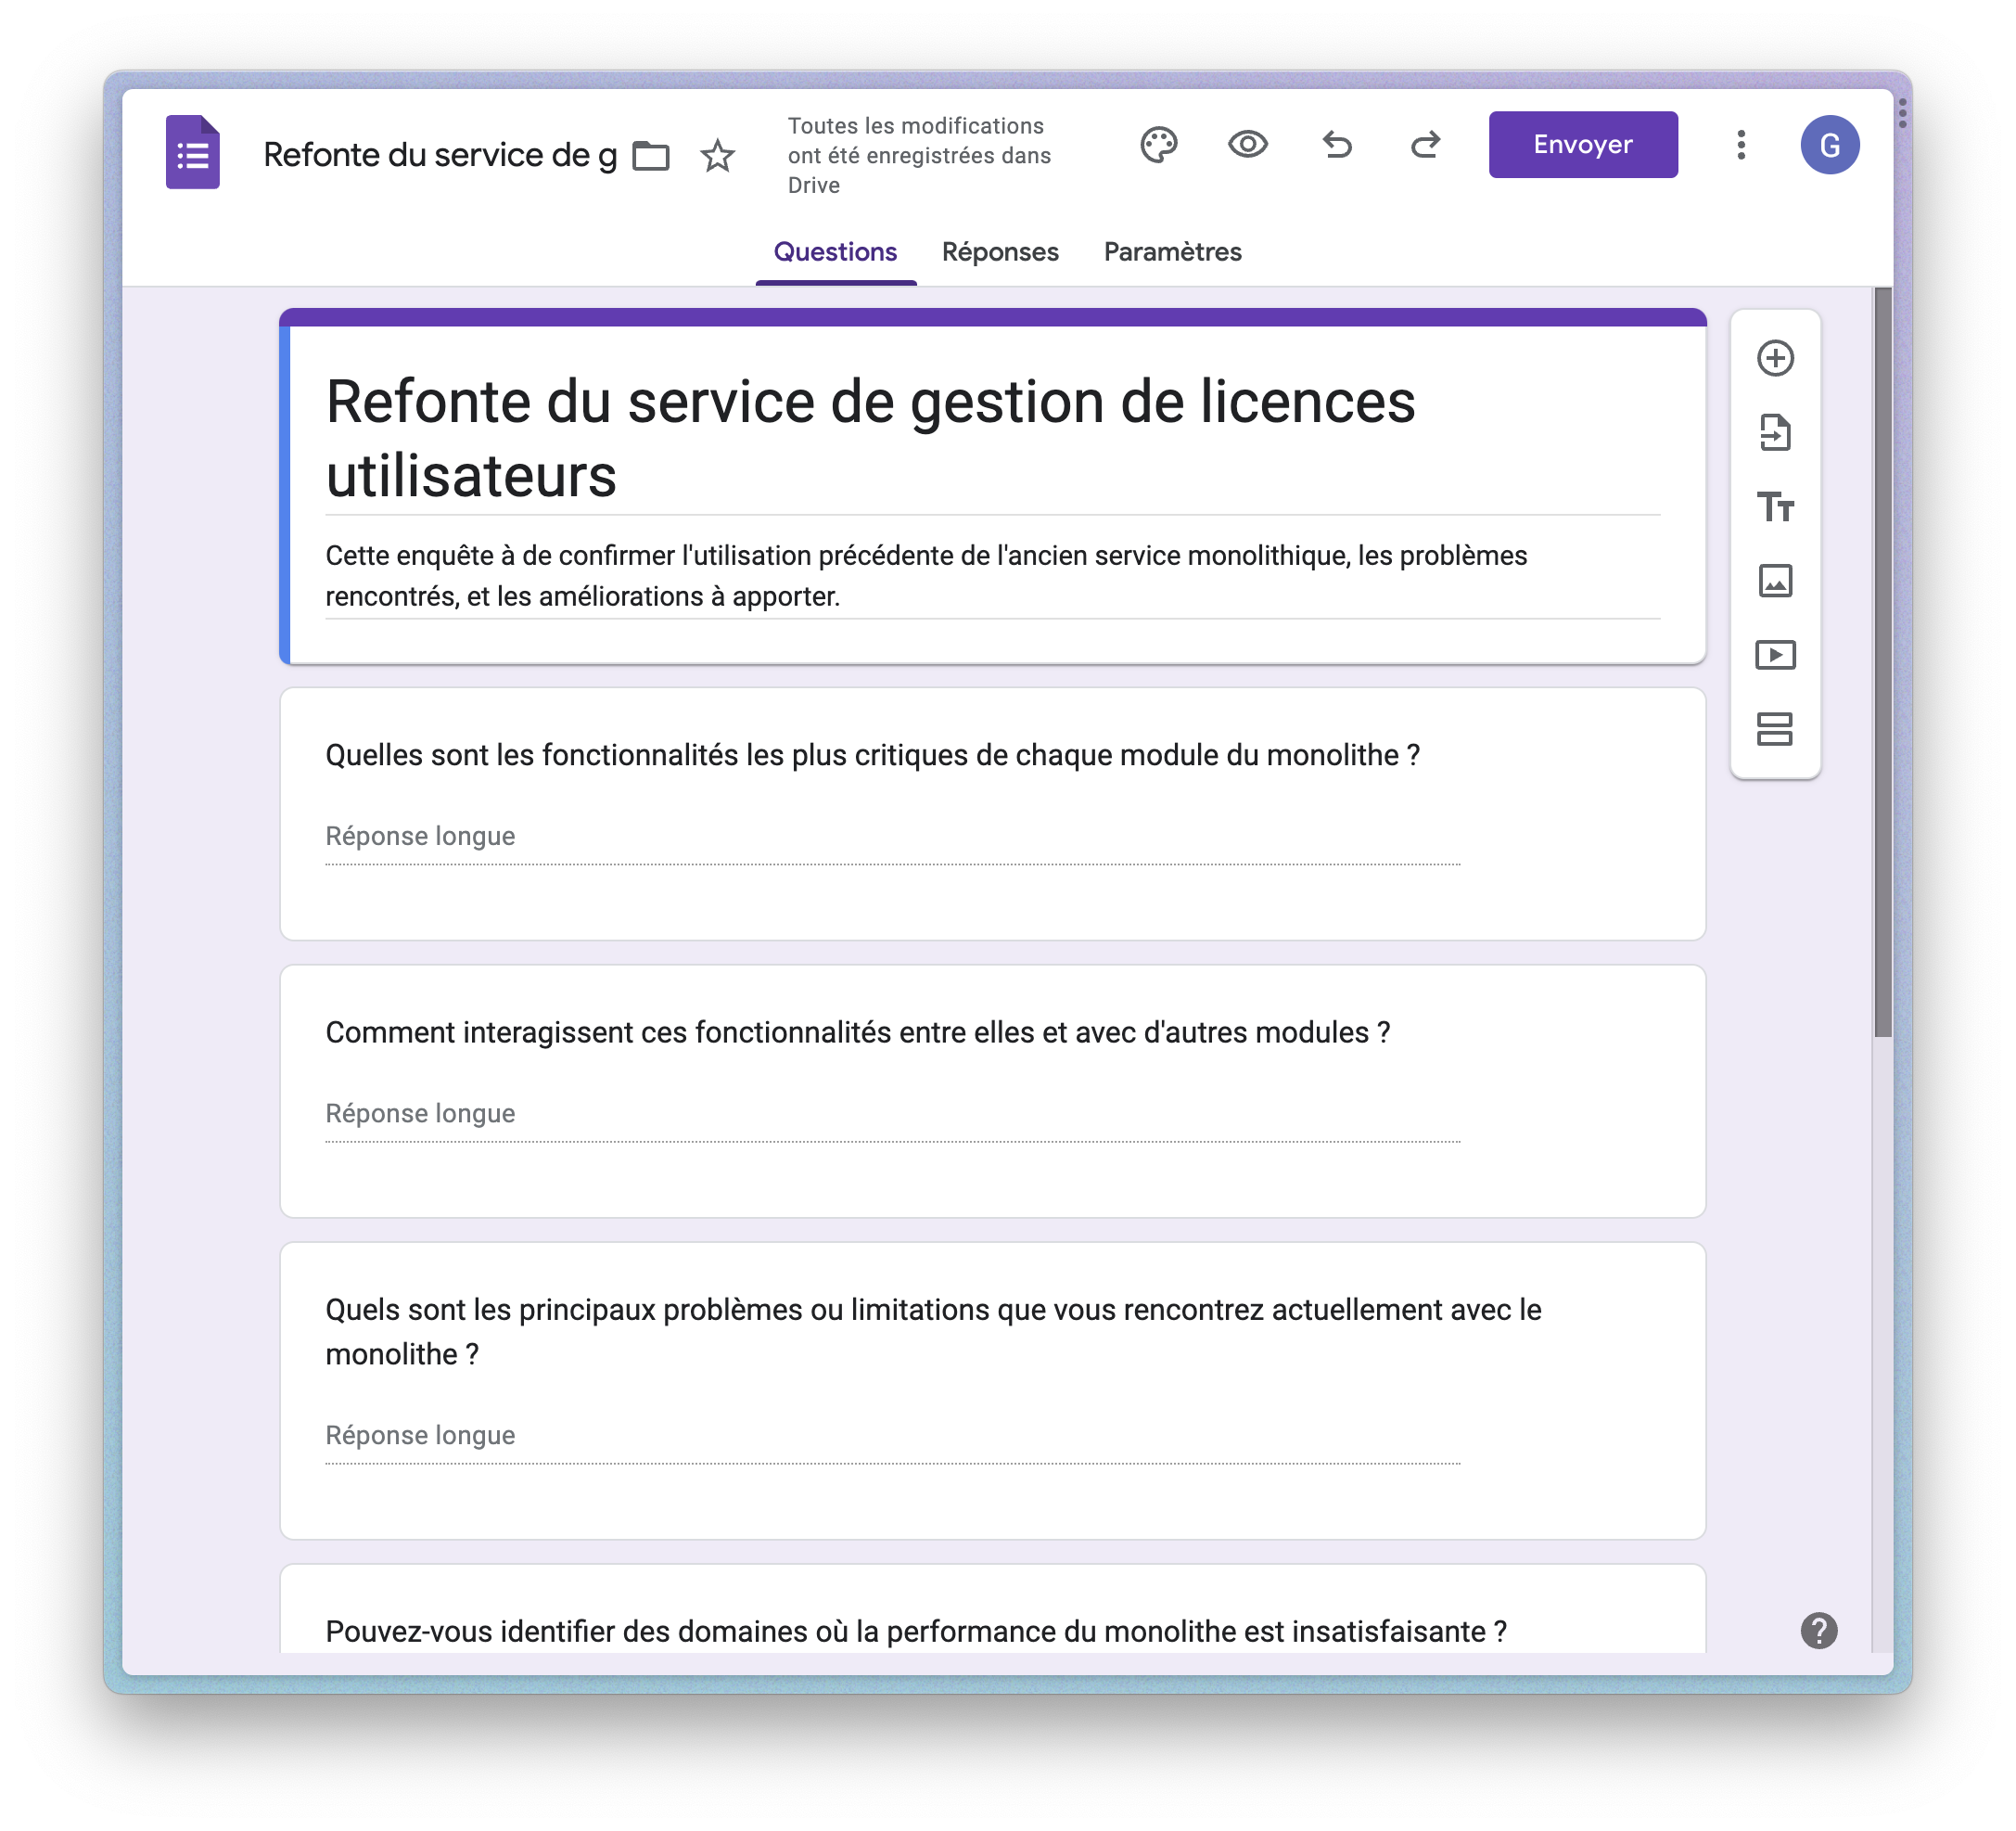
\includegraphics[scale=0.40,center]{screenshots/enquete-utilisateur.png}
      \caption{Google Forms pour la réalisation de l'enquête utilisateurs}
  \end{figure}
Les résultats sont présents sur l'onglet "Réponses", et ne sont visibles que par le créateur du Google Forms par défaut.
\subsubsection{Questions de l'enquête}
Voici une liste de 7 questions proposées aux trois développeurs ciblés, ces questions ayant pour but de confirmer l'utilisation précédente de l'ancien service monolithique, les problèmes rencontrés, et les améliorations à apporter.
\begin{enumerate}
\item Quelles sont les fonctionnalités les plus critiques de chaque module du monolithe ?
\item Comment interagissent ces fonctionnalités entre elles et avec d'autres modules ?
\item Quels sont les principaux problèmes ou limitations que vous rencontrez actuellement avec le monolithe ?
\item Pouvez-vous identifier des domaines où la performance du monolithe est insatisfaisante ?
\item Quels sont les éléments de sécurité importants à prendre en compte pour chaque module ?
\item Y a-t-il des fonctionnalités que vous souhaiteriez ajouter à chaque module à l'avenir ?
\item Quels sont les améliorations en terme d'UX/UI design que vous souhaiteriez rencontrer ?
\end{enumerate}
\subsection{Contexte de réalisation}
J'ai élaboré l'enquête en utilisant la plateforme Google Forms pour recueillir les informations nécessaires à la transformation du monolithe en microservices.
Les questions ont été formulées de manière à comprendre comment les utilisateurs interagissent avec le système et à identifier leurs préférences en matière de fonctionnalités.
Toute cette compétence à été réalisée à distance avec des outils de travail collaboratif en ligne, comme Microsoft Teams, pour communiquer avec les différents collaborateurs.
Une réunion finale a eu lieu pour partager les résulats de l'enquête aux différents membres de l'équipe R\&D, pour valider les réponses et propositions de chacun.
\subsection{Conclusion sur l'activité}
Cette compétence n'a pas à mon avis d'évolution majeure à venir dans les 10 ans à venir, la plus grande dernièrement étant le passage du papier au numérique pour la réaliser.
\newline
\newline
Je n'ai pas eu de difficulé particulière quand à la réalisation de cette compétence, et je ne vois non plus de piste de progression.

\section{Activité 5 - conception d'une architecture applicative évolutive et tolérante aux pannes}
\subsection{Compétence et son fondement}
\textbf{Bloc de compétences}: A5 – Développement d’une solution applicative spécifique et métier selon le projet de développement S.I.
\newline
\textbf{Compétence choisie}: A5C2 – Concevoir une architecture applicative selon la complexité du système d’information existant de type architecture distribuée, ou micro service évolutive et tolérante aux pannes
\newline
\textbf{Détails}: Cette compétence consiste à démontrer ma capacité à proposer une architecture applicative :
\begin{itemize}
  \item argumenter mon choix en formalisant par écrit les critères de stabilité, d’efficacité et
de pérennité.
  \item lister l’environnement technique adéquat à son architecture applicative (architecture distribuée, clusters,architecture micro services, REST, appel des services....)
  \item présenter sous forme de schéma la logique du fonctionnement de notre architecture applicative
\end{itemize}
\subsection{Présentation et réalisation de l'activité}
\subsubsection{Analyse en amont de la réalisation du schéma d'infrastructure}
Étant déjà dans une architecture en microservices avec Qibates,
j'ai choisis de continuer sur cette architecture, en rajoutant les nouveaux services créés depuis l'ancien service monolithique.
J'ai décomposé les principaux points à prendre en compte, que voici:
\begin{enumerate}
\item \textbf{Analyse des Besoins} : J'ai commencé par examiner les besoins spécifiques de l'application,
  en mettant l'accent sur la séparation des fonctionnalités en modules indépendants et en 
  identifiant les services critiques.
\item \textbf{Décomposition des Fonctionnalités} : J'ai découpé
  l'application monolithe en modules autonomes, chacun représentant une
  fonctionnalité ou un domaine spécifique. Chaque module serait
  développé et déployé en tant que service indépendant.
\item \textbf{Choix Technologiques} : J'ai sélectionné les technologies
  appropriées pour la mise en œuvre de l'architecture microservices.
J'ai opté pour Spring Boot pour le développement des services REST et
  Angular pour l'interface utilisateur.
\item \textbf{Communication entre Services} : J'ai mis en place des API REST
  pour permettre la communication entre les différents services. J'ai
  également utilisé un système de messagerie pour les notifications
  asynchrones entre les services lorsque nécessaire.
\item \textbf{Gestion des Erreurs et Tolérance aux Pannes} : J'ai intégré
  des mécanismes de gestion des erreurs tels que les messages d'erreur
  standardisés et les codes d'état HTTP. De plus, j'ai conçu des
  stratégies de récupération pour garantir la continuité du service en
  cas de défaillance d'un module.
\item \textbf{Équilibrage de Charge} : J'ai mis en place un équilibrage de
  charge pour répartir les requêtes entre les différents services,
  assurant ainsi une utilisation optimale des ressources et une
  meilleure réactivité de l'application.
\item \textbf{Sécurité} : J'ai intégré des mécanismes de sécurité tels que
  l'authentification et l'autorisation au niveau des services, ainsi
  qu'une API Gateway (en utilisant notre serveur Nginx existant)
  pour centraliser la gestion des accès.
\item \textbf{Monitoring et Journalisation} : J'ai inclus des outils de
  supervision pour surveiller les performances et la disponibilité des
  services. J'ai également configuré la journalisation pour faciliter le
  débogage en cas de problème. Telegraf est utilisé pour récupérer les métriques,
  InfluxDB pour les stocker, et Grafana pour les afficher. Ces trois solutions sont
  open-sources.
\item \textbf{Documenter l'Architecture} : J'ai préparé une documentation
  détaillée de l'architecture, y compris les interactions entre les
  services, les dépendances, les flux de données et les points d'entrée.
\item \textbf{Validation et Tests} : J'ai testé l'architecture en simulant
  différentes conditions, notamment des pannes de services et des pics
  de charge, pour m'assurer de sa stabilité et de sa capacité à répondre
  aux besoins. L'utilisant en interne pour d'autres projets, j'ai utilisé Jmeter, une solution open-source,
  pour effectuer ces tests de charge.
\end{enumerate}
\subsubsection{Réalisation du schéma d'infrastructure}
  \begin{figure}[H]
      \centering
      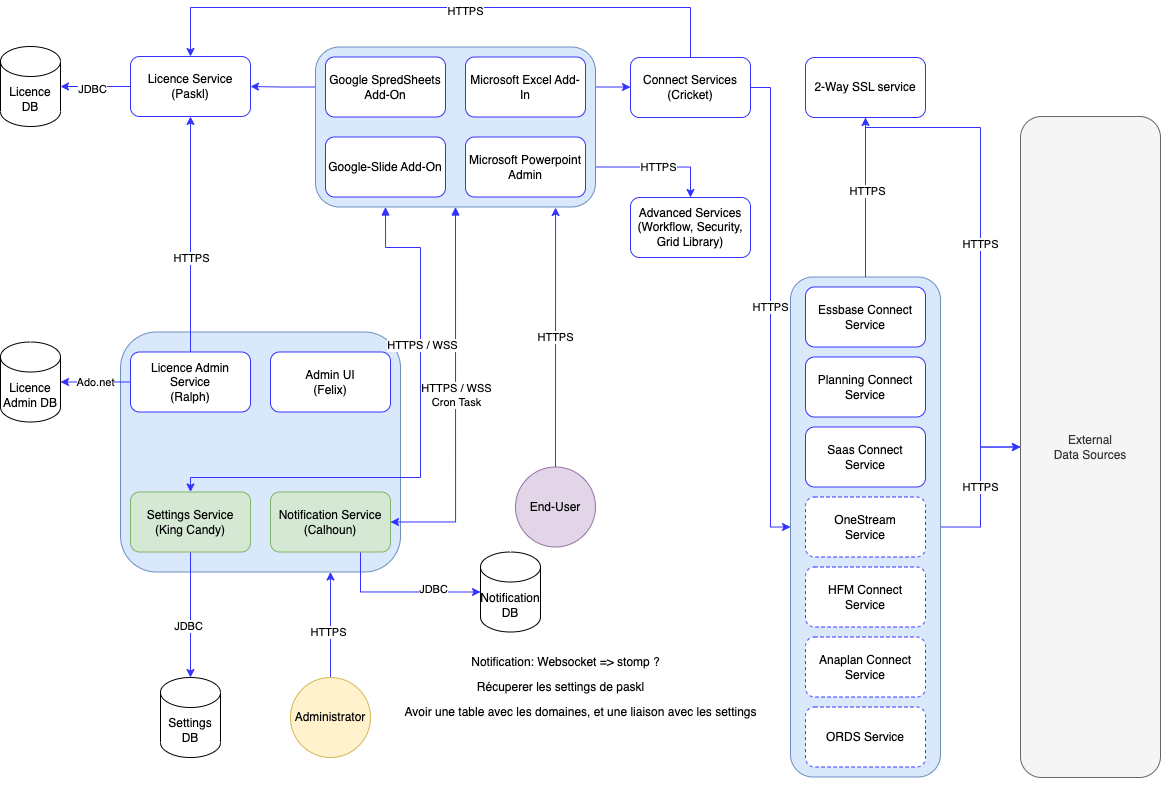
\includegraphics[scale=0.40,center]{schemas/schema-qibates-v2.png}
      \caption{Schéma de la refonte en microservices}
  \end{figure}
Voici donc le nouveau schéma de l'architecture de QiBates. La zone bleu
en bas à gauche, ainsi que les bases de données liées aux microservices
dans cette zone, sont les nouveaux microservices remplaçant l'ancien
service monolithique.
\newline
Le service ``\textbf{Admin UI}'' est l'interface web permettant de gérer
les 3 autres microservices liés.
\newline
``\textbf{Licence Admin}'' permet comme son nom l'indique de gérer les
licences utilisateurs des clients, pour utiliser QiBates.
\newline
``\textbf{Settings Service}'' permet à un utilisateur de sauvegarder des
paramètres pour QiBates comme bon lui semble.
\newline
``\textbf{Notification Service}'' permet l'envoie de notifications à un
utilisateur, comme par exemple une notification de fin de tâche de
calcul sur QiBates.
\newline
\newline
L'interface d'administration est une application web, les 3 autres services sont des API REST,
et PostgreSQL est utilisé comme SGBD pour les bases de données.
Toutes les communications entre chaque service utilisent le protocole HTTP.
\subsection{Contexte de réalisation}
J'ai utilisé Draw.io, un logiciel gratuit et open-source pour réaliser les schémas d'architecture.
J'ai aussi utilisé Microsoft Teams pour valider mes schémas auprès de mon directeur technique, lors de réunions en visioconférences.
\subsection{Conclusion sur l'activité}
Dans 10 ans, les architectures micro-services seront toujours présentes, même si celle-ci a des problèmes liés aux coûts qui peuvent se montrer excessif, malgré un avantage certain quand à la réduction de complexité et une augmentation de la fiabilité par rapport à une architecture monolithique.
\newline
\newline
Ayant travaillé précédemment sur d'autres microservices de QiBates, je n'ai pas rencotré de difficulté partifuclière quand à la réalisation de cette activité.
Le choix des technologies a été effectué en prenant en compte l'architecture actuelle, et les moyens de communications entre microservices sont basés sur les standards du web (émis par la W3C).

\section{Activité 6 - développement d'une application pour répondre aux besoins utilisateurs/directions métiers}
\subsection{Compétence et réalisation et son fondement}
\textbf{Bloc de compétences}: A5 – Développement d’une solution applicative spécifique et métier selon le projet de développement S.I.
\newline
\textbf{Compétence choisie}: A5C3 Développer une application adéquate selon la stratégie applicative de l’environnement en utilisant un langage de programmation approprié dans le respect du cahier des charges établi afin de répondre aux besoins utilisateurs/directions métiers
\newline
\textbf{Détails}: Cette compétence consiste à démontrer ma capacité à développer une application en
adéquation avec l’environnement technique de l’entreprise (développement web, développement mobile, développement embarqué, développement IOT) :
\begin{itemize} 
 \item utiliser le langage de programmation approprié à l’environnement technique
 \item concevoir et détaille une logique de développement dans le respect du cahier des charges
 \item en résultat attendu, faire une démonstration technique de l'application (interprétation de certaines lignes de codes)
\end{itemize}
\subsection{Présentation et réalisation de l'activité}
\subsubsection{Introduction}
Pour développer les microservices, j'ai utilisé Angular pour réaliser
l'interface web, Spring Boot pour les API REST, et PostgreSQL comme
SGBD. Ces technologies sont déjà utilisées pour nos microservices
précédents, j'ai choisis de les réutiliser, car ayant déjà des
connaissance avec, je peux aussi demander de l'aide aux autres
collaborateurs en cas de problème, et notre stack technologique est
uniforme dans notre infrastructure.

\textbf{Angular} est un framework web utilisant TypeScript, conçu pour
créer des applications interactives et dynamiques côté client. Il
facilite la gestion des composants, de l'état de l'application et des
interactions avec les données.

\textbf{Spring Boot} est un framework Java qui simplifie la création
d'applications robustes et évolutives en gérant automatiquement la
configuration et en fournissant des fonctionnalités prêtes à l'emploi,
comme la création de routes pour une API REST, un $\emph{ORM}^{12}$, et des outils
pour tester notre code.

\textbf{PostgreSQL} est un système de gestion de base de données
relationnelle open source, permettant de stocker et d'organiser des
données de manière structurée, et sa fiabilité n'est plus à démontrer.
\subsubsection{Structure des projets}
  \begin{figure}[H]
      \centering
      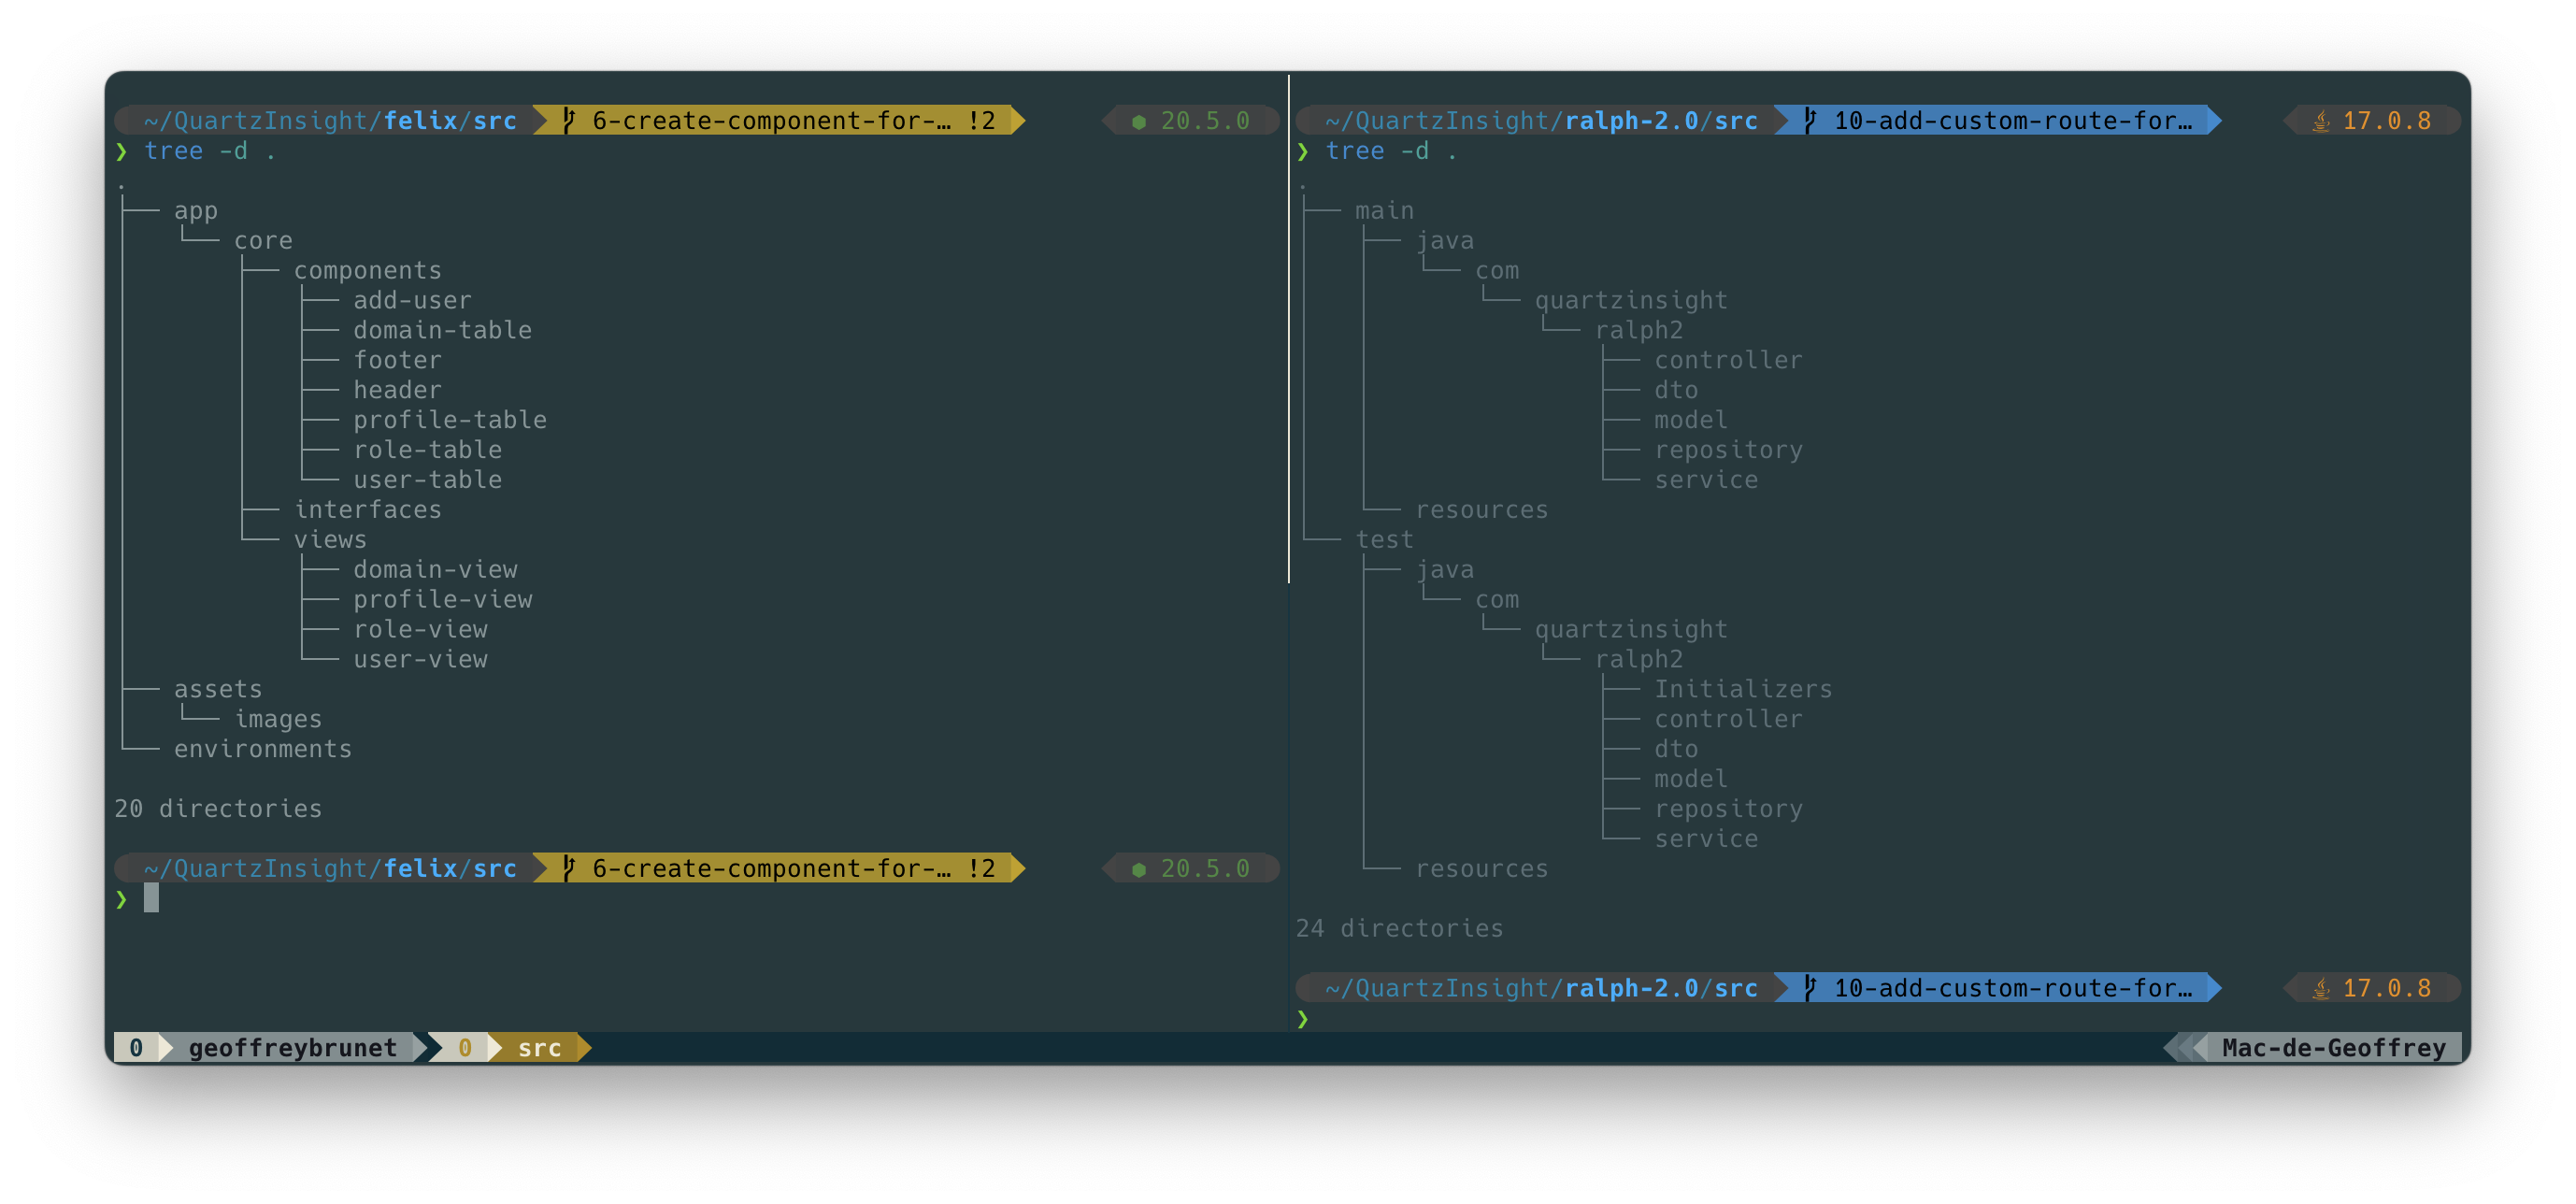
\includegraphics[scale=0.35,center]{screenshots/directories.png}
      \caption{Structure des dossiers pour deux microservices}
  \end{figure}
J'ai utilisé la structure commune aux projets Spring Boot, pour une
meilleure compréhension, une meilleure collaboration et une meilleure
maintenance:

\begin{enumerate}
\def\labelenumi{\arabic{enumi}.}
\tightlist
\item
  \textbf{main}

  \begin{itemize}
  \tightlist
  \item
    \textbf{java}: C'est ici que se trouve le code Java principal de
    l'application.

    \begin{itemize}
    \tightlist
    \item
      \textbf{com.quartzinsight.ralph2.TITI}: C'est le package de base
      de l'application.

      \begin{itemize}
      \tightlist
      \item
        \textbf{controller}: Contient les classes qui gèrent les
        requêtes HTTP.
      \item
        \textbf{model}: Contient les classes représentant les entités de
        données de l'application.
      \item
        \textbf{repository}: Contient les interfaces pour interagir avec
        la base de données.
      \item
        \textbf{service}: Contient la logique métier de l'application.
      \end{itemize}
    \end{itemize}
  \end{itemize}
\item
  \textbf{resources}: Contient les fichiers de configuration et les
  ressources statiques de l'application.
\end{enumerate}

J'ai aussi utilisé la même structure pour l'application Angular que dans
la documentation officielle:

\begin{itemize}
\tightlist
\item
  \textbf{app}: C'est le répertoire principal de l'application.

  \begin{itemize}
  \tightlist
  \item
    \textbf{core}: Contient les éléments centraux de l'application tels
    que les services partagés et les intercepteurs HTTP.
  \item
    \textbf{components}: Contient les composants réutilisables de
    l'application.

    \begin{itemize}
    \tightlist
    \item
      \textbf{add-user}: Un composant pour ajouter un nouvel
      utilisateur.
    \item
      \textbf{domain-table}: Un composant pour afficher un tableau de
      domaines.
    \item
      \textbf{footer}: Un composant pour le pied de page.
    \item
      \textbf{header}: Un composant pour l'en-tête.
    \item
      \textbf{profile-table}: Un composant pour afficher un tableau de
      profils.
    \item
      \textbf{role-table}: Un composant pour afficher un tableau de
      rôles.
    \item
      \textbf{user-table}: Un composant pour afficher un tableau
      d'utilisateurs.
    \end{itemize}
  \item
    \textbf{interfaces}: Contient les interfaces TypeScript utilisées
    dans l'application.
  \item
    \textbf{views}: Contient les vues principales de l'application.

    \begin{itemize}
    \tightlist
    \item
      \textbf{domain-view}: Une vue pour afficher les détails d'un
      domaine.
    \item
      \textbf{profile-view}: Une vue pour afficher les détails d'un
      profil.
    \item
      \textbf{role-view}: Une vue pour afficher les détails d'un rôle.
    \item
      \textbf{user-view}: Une vue pour afficher les détails d'un
      utilisateur.
    \end{itemize}
  \end{itemize}
\item
  \textbf{assets}: Contient les ressources statiques de l'application,
  comme les images.
\item
  \textbf{environments}: Contient les fichiers de configuration pour
  différents environnements (par exemple, développement et production).
\end{itemize}
\subsubsection{Exemple de code}
  \begin{figure}[H]
      \centering
      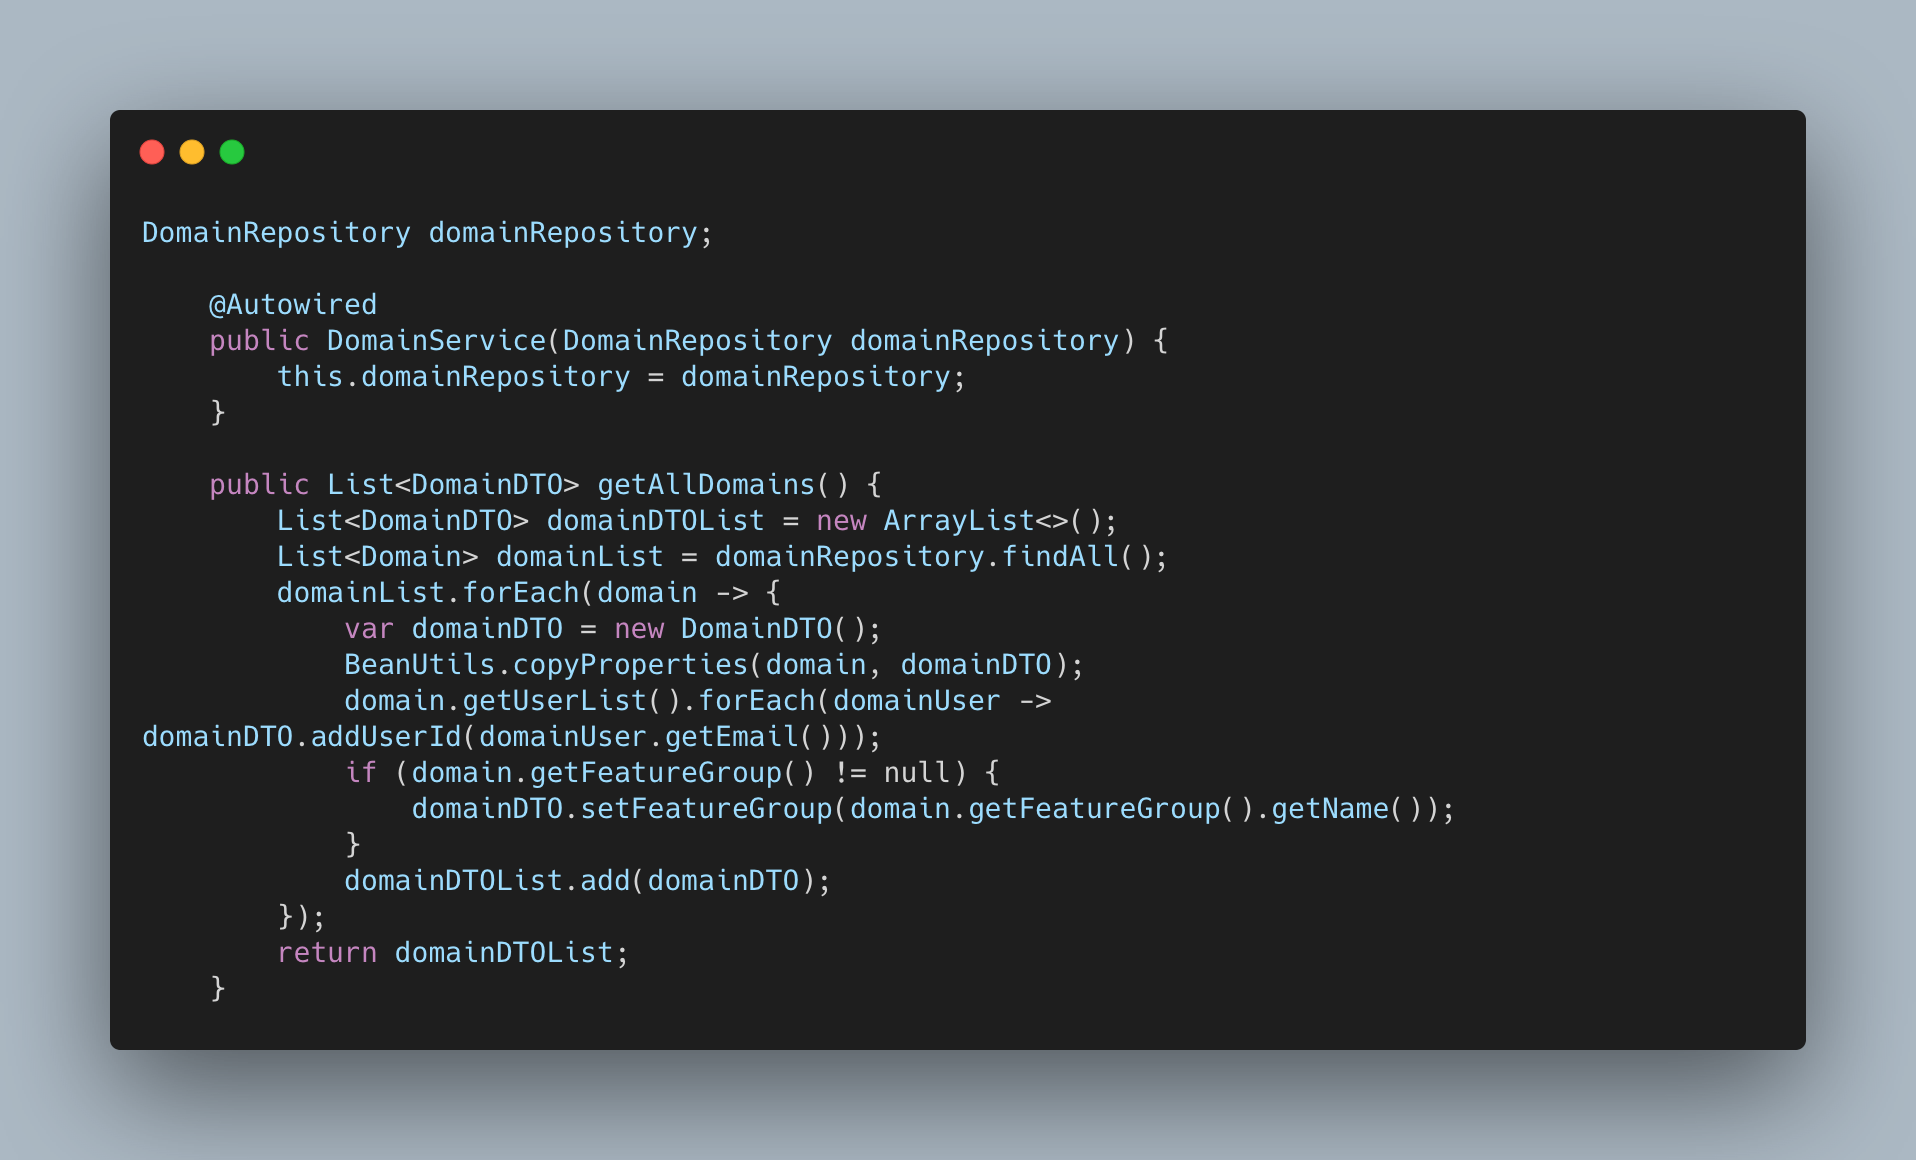
\includegraphics[scale=0.40,center]{screenshots/java-code.png}
      \caption{Exemple de code d'un service Spring Boot renvoyant une liste de domaines}
  \end{figure}
Ce code utilise l'annotation Spring \texttt{@Autowired} pour injecter une instance
de \texttt{DomainRepository} dans le service \texttt{DomainService}. Ce
service récupère tous les domaines à partir de la base de données en
utilisant la méthode \texttt{findAll()} du repository. Ensuite, pour
chaque domaine, il crée un objet \texttt{DomainDTO} (Data Transfer
Object), qui est une structure pour transporter les données. Les
propriétés du domaine sont copiées vers le DTO à l'aide de
\texttt{BeanUtils.copyProperties()}. En outre, les ID des utilisateurs
associés sont ajoutés au DTO, et si le domaine a un groupe de
fonctionnalités, le nom du groupe est défini dans le DTO. En fin de
compte, une liste de DTOs de domaine est renvoyée.
  \begin{figure}[H]
      \centering
      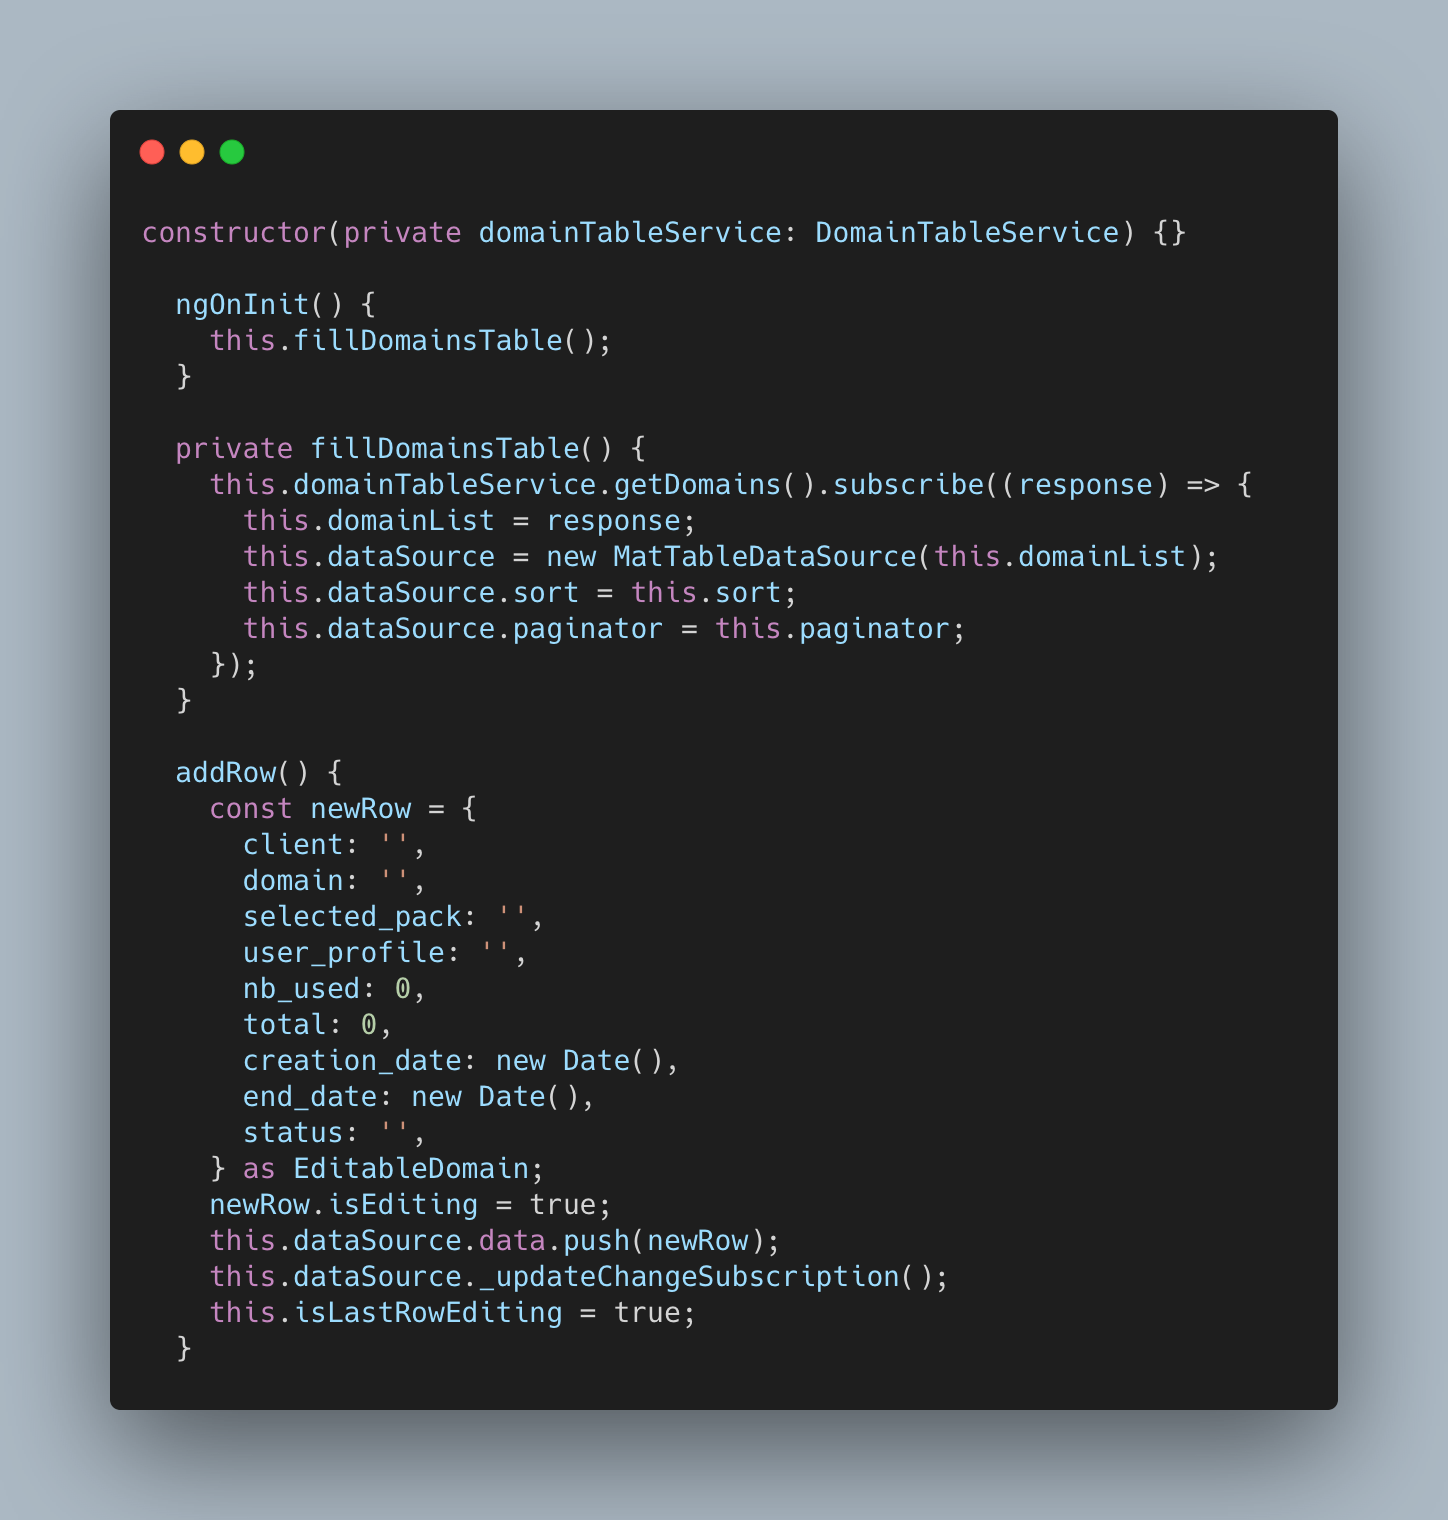
\includegraphics[scale=0.40,center]{screenshots/js-code.png}
      \caption{Exemple de code d'un service Spring Boot renvoyant une liste de domaines}
  \end{figure}
Ce code Angular exécute les actions suivantes :
\begin{enumerate}
\def\labelenumi{\arabic{enumi}.}
\item
  Dans la méthode \texttt{ngOnInit()}, au démarrage du composant,
  \texttt{fillDomainsTable()} est appelée pour remplir une table de
  données de domaines.
\item
  La fonction \texttt{fillDomainsTable()} utilise
  \texttt{domainTableService} pour obtenir des domaines via une requête
  asynchrone. Une fois la réponse reçue, elle configure une source de
  données de table (\texttt{MatTableDataSource}) avec les domaines pour
  permettre le tri et la pagination.
\item
  \texttt{addRow()} ajoute une nouvelle ligne à la table. Elle crée un
  nouvel objet avec des valeurs par défaut, le marque comme en cours
  d'édition, et l'ajoute à la liste des données de la table. Ensuite, la
  table est mise à jour pour refléter cette modification. Cette fonction
  est utilisée pour ajouter de nouvelles entrées à une table éditable.
\end{enumerate}
\subsection{Contexte de réalisation}
J'ai utilisé \textbf{Neovim} comme éditeur de code, \textbf{Maven} comme gestionnaire de builds et dépendances pour les microservices en Java (Version 17), et \textbf{Node.JS} / \textbf{NPM} comme runtime et gestionnaire de dépendances pour l'application Angular.
\subsection{Conclusion sur l'activité}
Cette compétence m'a permit de m'améliorer sur le développement, et de collaborer en équipe pour que les microservices soient en adéquation avec notre architecture actuelle et répondent aux besoins des utilisateurs.
\newline
\newline
Le choix des technologies et langages est sujet à fort changement, en effet, depuis 10 ans, les technologies utilisées ont bien changées, et certaines comme Angular n'existaient pas.

\section{Activité 7 - analyse de la qualité de la solution applicative et mise en place d’un plan de correction / d’amélioration}
\subsection{Compétence et son fondement}
\textbf{Bloc de compétences}: A5 – Développement d’une solution applicative spécifique et métier selon le projet de développement S.I.
\newline
\textbf{Compétence choisie}: A5C5 – Effectuer les tests de la solution applicative paramétrée ou développée pour identifier les erreurs et dysfonctionnements et établir les plans de correction/d’amélioration avant sa mise en production
\newline
\textbf{Détails}: Cette compétence consiste à démonter ma capacité à tester une solution applicative :
\begin{itemize}
  \item rédiger un plan de test en précisant la typologie de test (unitaire, recette, d’intégration), les données de test et les résultats attendus
  \item mettre en œuvre le plan de test à l’aide des jeux d’essai
  \item utiliser un outil de testing de mon choix
  \item Résultat attendu : présenter les facteurs de la bonne testabilité de son plan de test
\end{itemize}
\subsection{Présentation et réalisation de l'activité}
Pour vérifier la qualité de mon code, j'écrit des tests unitaires et
d'intégration. Nous utilisons en interne un outil appelé SonarQube pour
vérifier la qualité de notre code. Voici un exemple d'un test unitaire
pour l'application Angular, ainsi que la page SonarQube associé à cette
même application.
  \begin{figure}[H]
      \centering
      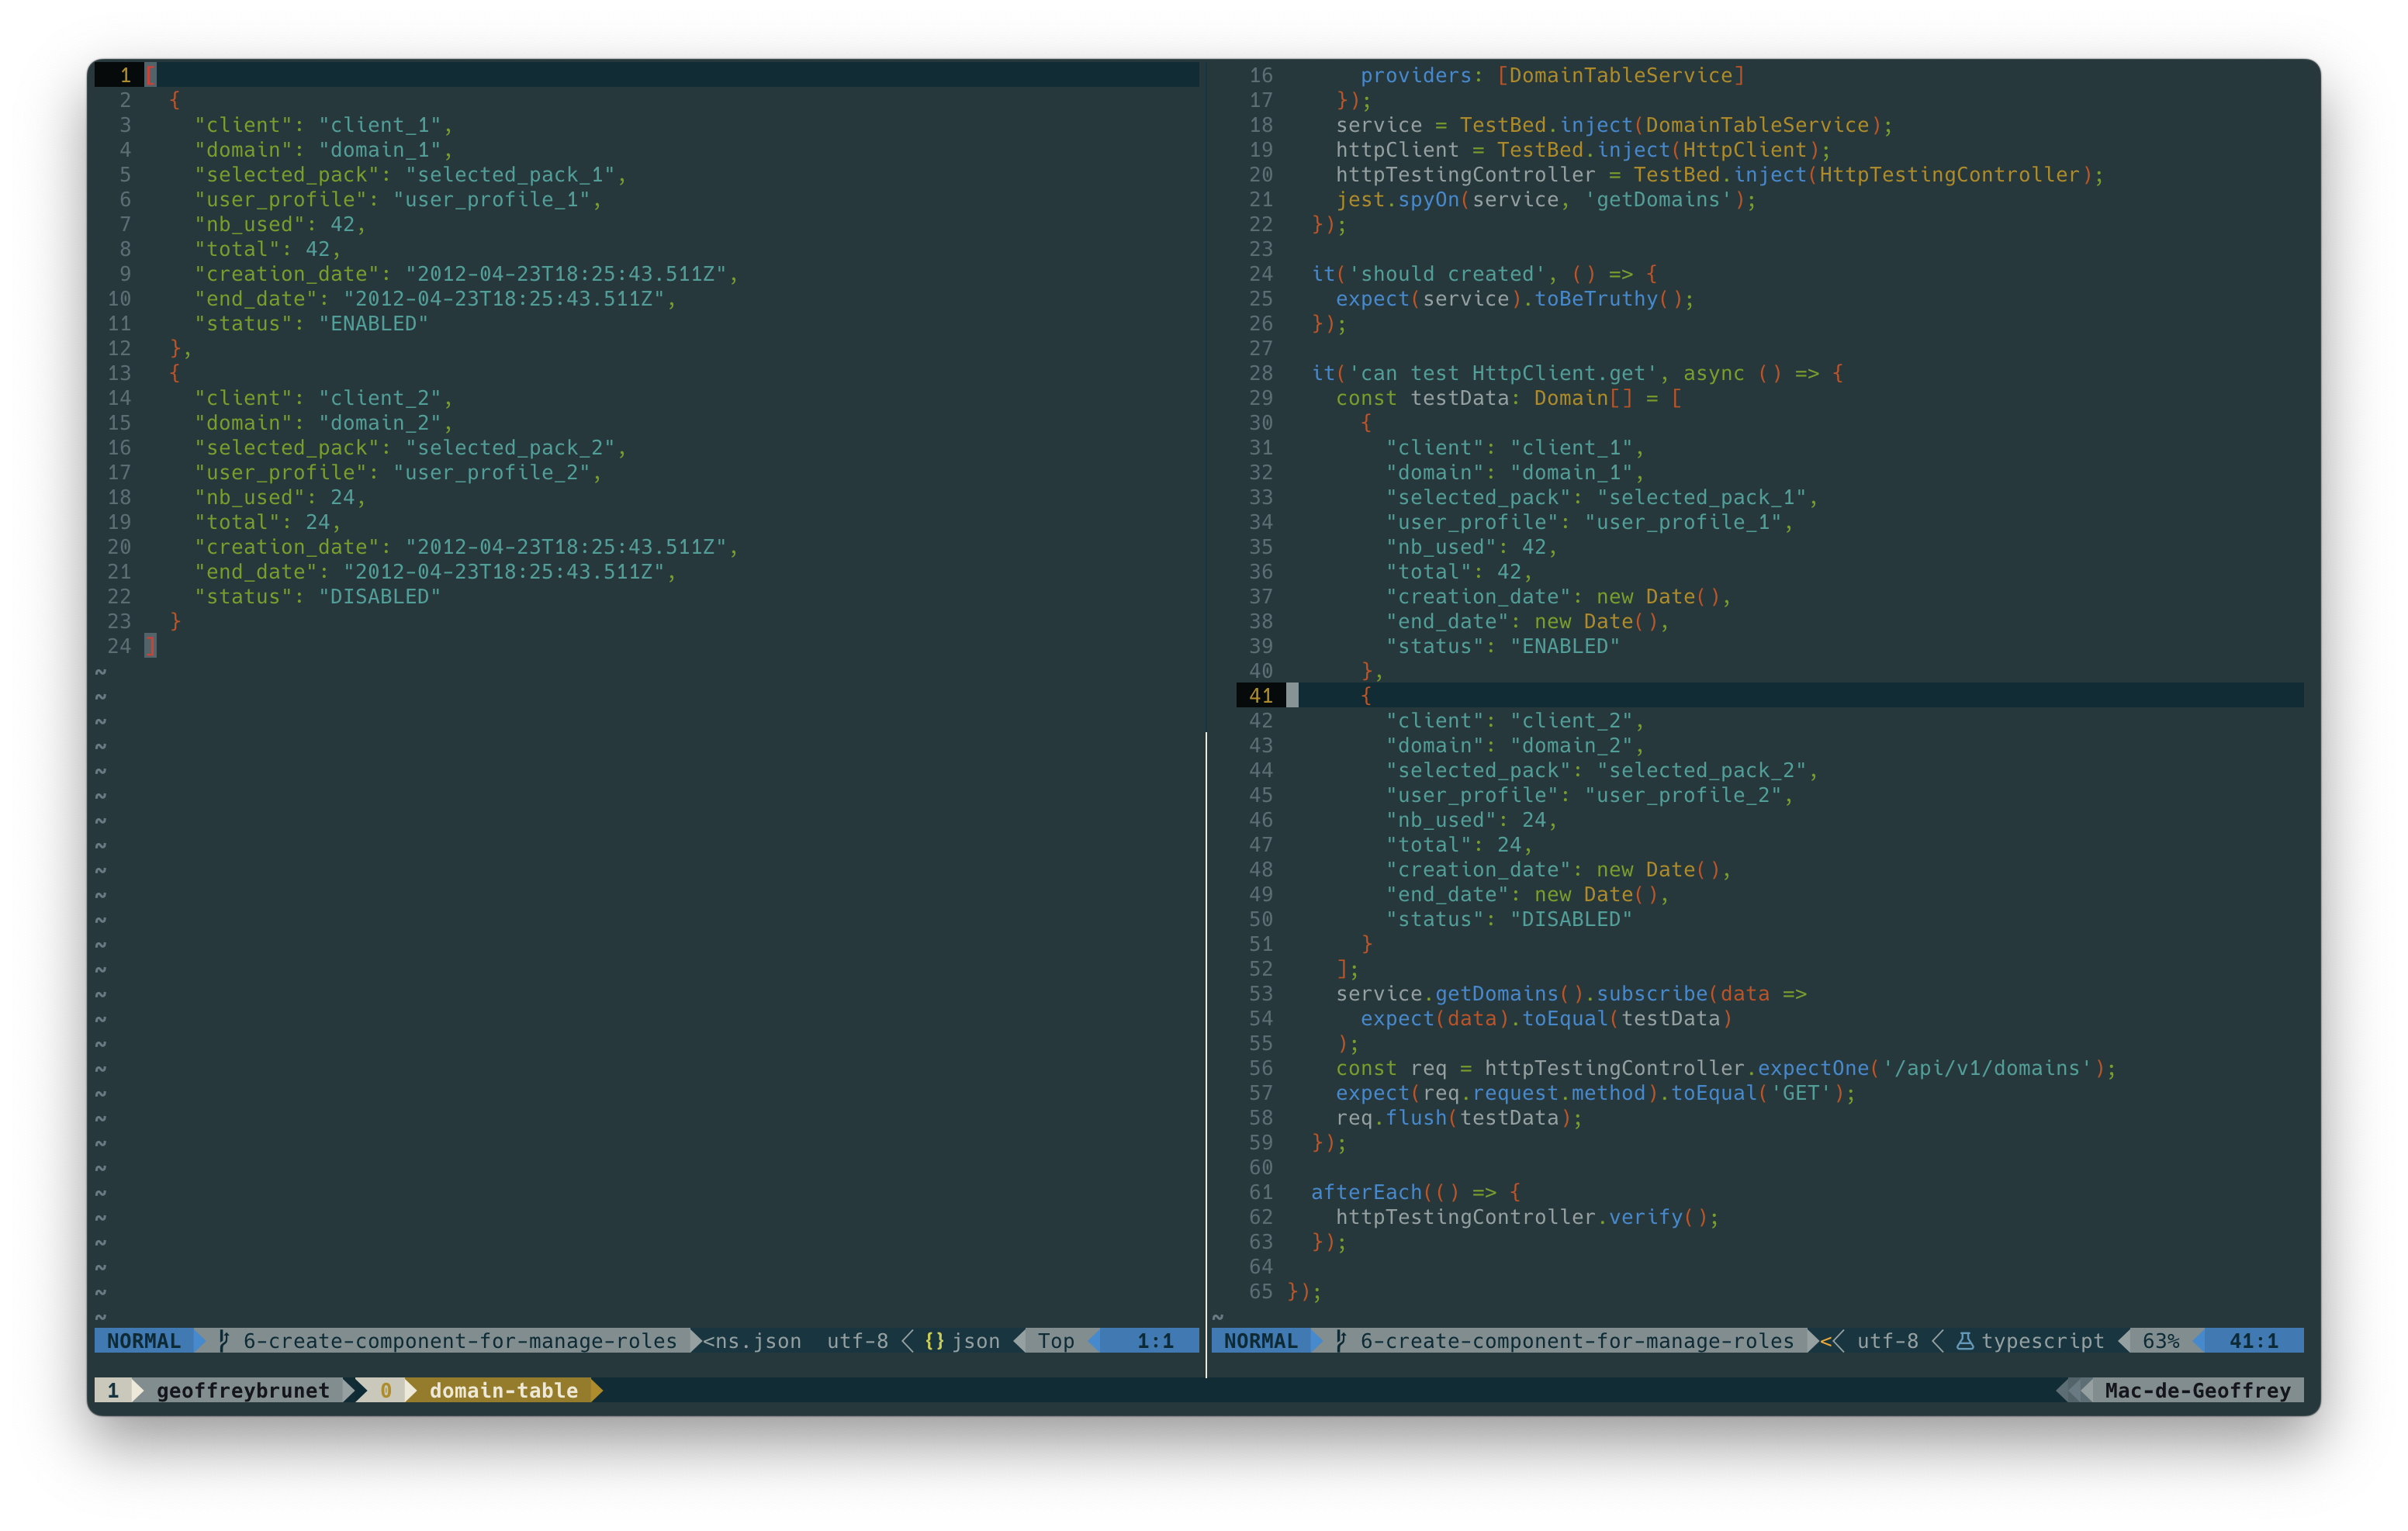
\includegraphics[scale=0.35,center]{screenshots/felix-test.png}
      \caption{Exemple de fausses données et d'un test unitaire les utilisant}
  \end{figure}
Ce code comprend des tests unitaires pour un service. Dans le premier
test, il vérifie si le service a été créé avec succès en utilisant le
fournisseur \texttt{DomainTableService}. Ensuite, il simule
l'utilisation de MirageJs pour gérer les requêtes HTTP en simulant des
données de domaine similaires à ``client'': ``client 1'', ``domain'':
``domain\_1'', etc. Dans le deuxième test, il vérifie si le service
\texttt{getDomains()} est appelé à l'aide de \texttt{jest.spyOn()}. Le
code utilise également \texttt{httpTestingController} pour simuler les
requêtes HTTP et compare les données reçues avec les données de test
définies. L'ensemble des tests est exécuté dans un environnement de test
Angular grâce à \texttt{TestBed}.
\newline
\newline
\textbf{MirageJS} est une bibliothèque JavaScript qui permet de simuler
des appels API HTTP côté client lors des tests. Elle est
particulièrement utile pour les tests unitaires et d'intégration, car
elle permet de créer un faux backend et de définir des endpoints avec
des données simulées, évitant ainsi les appels réels aux serveurs et les
dépendances externes.

Pour les tests sur les API REST, j'utilise des ``mocks'', des
simulations de requêtes HTTP, grâce aux outils présents nativement dans
Spring Starter Test.
  \begin{figure}[H]
      \centering
      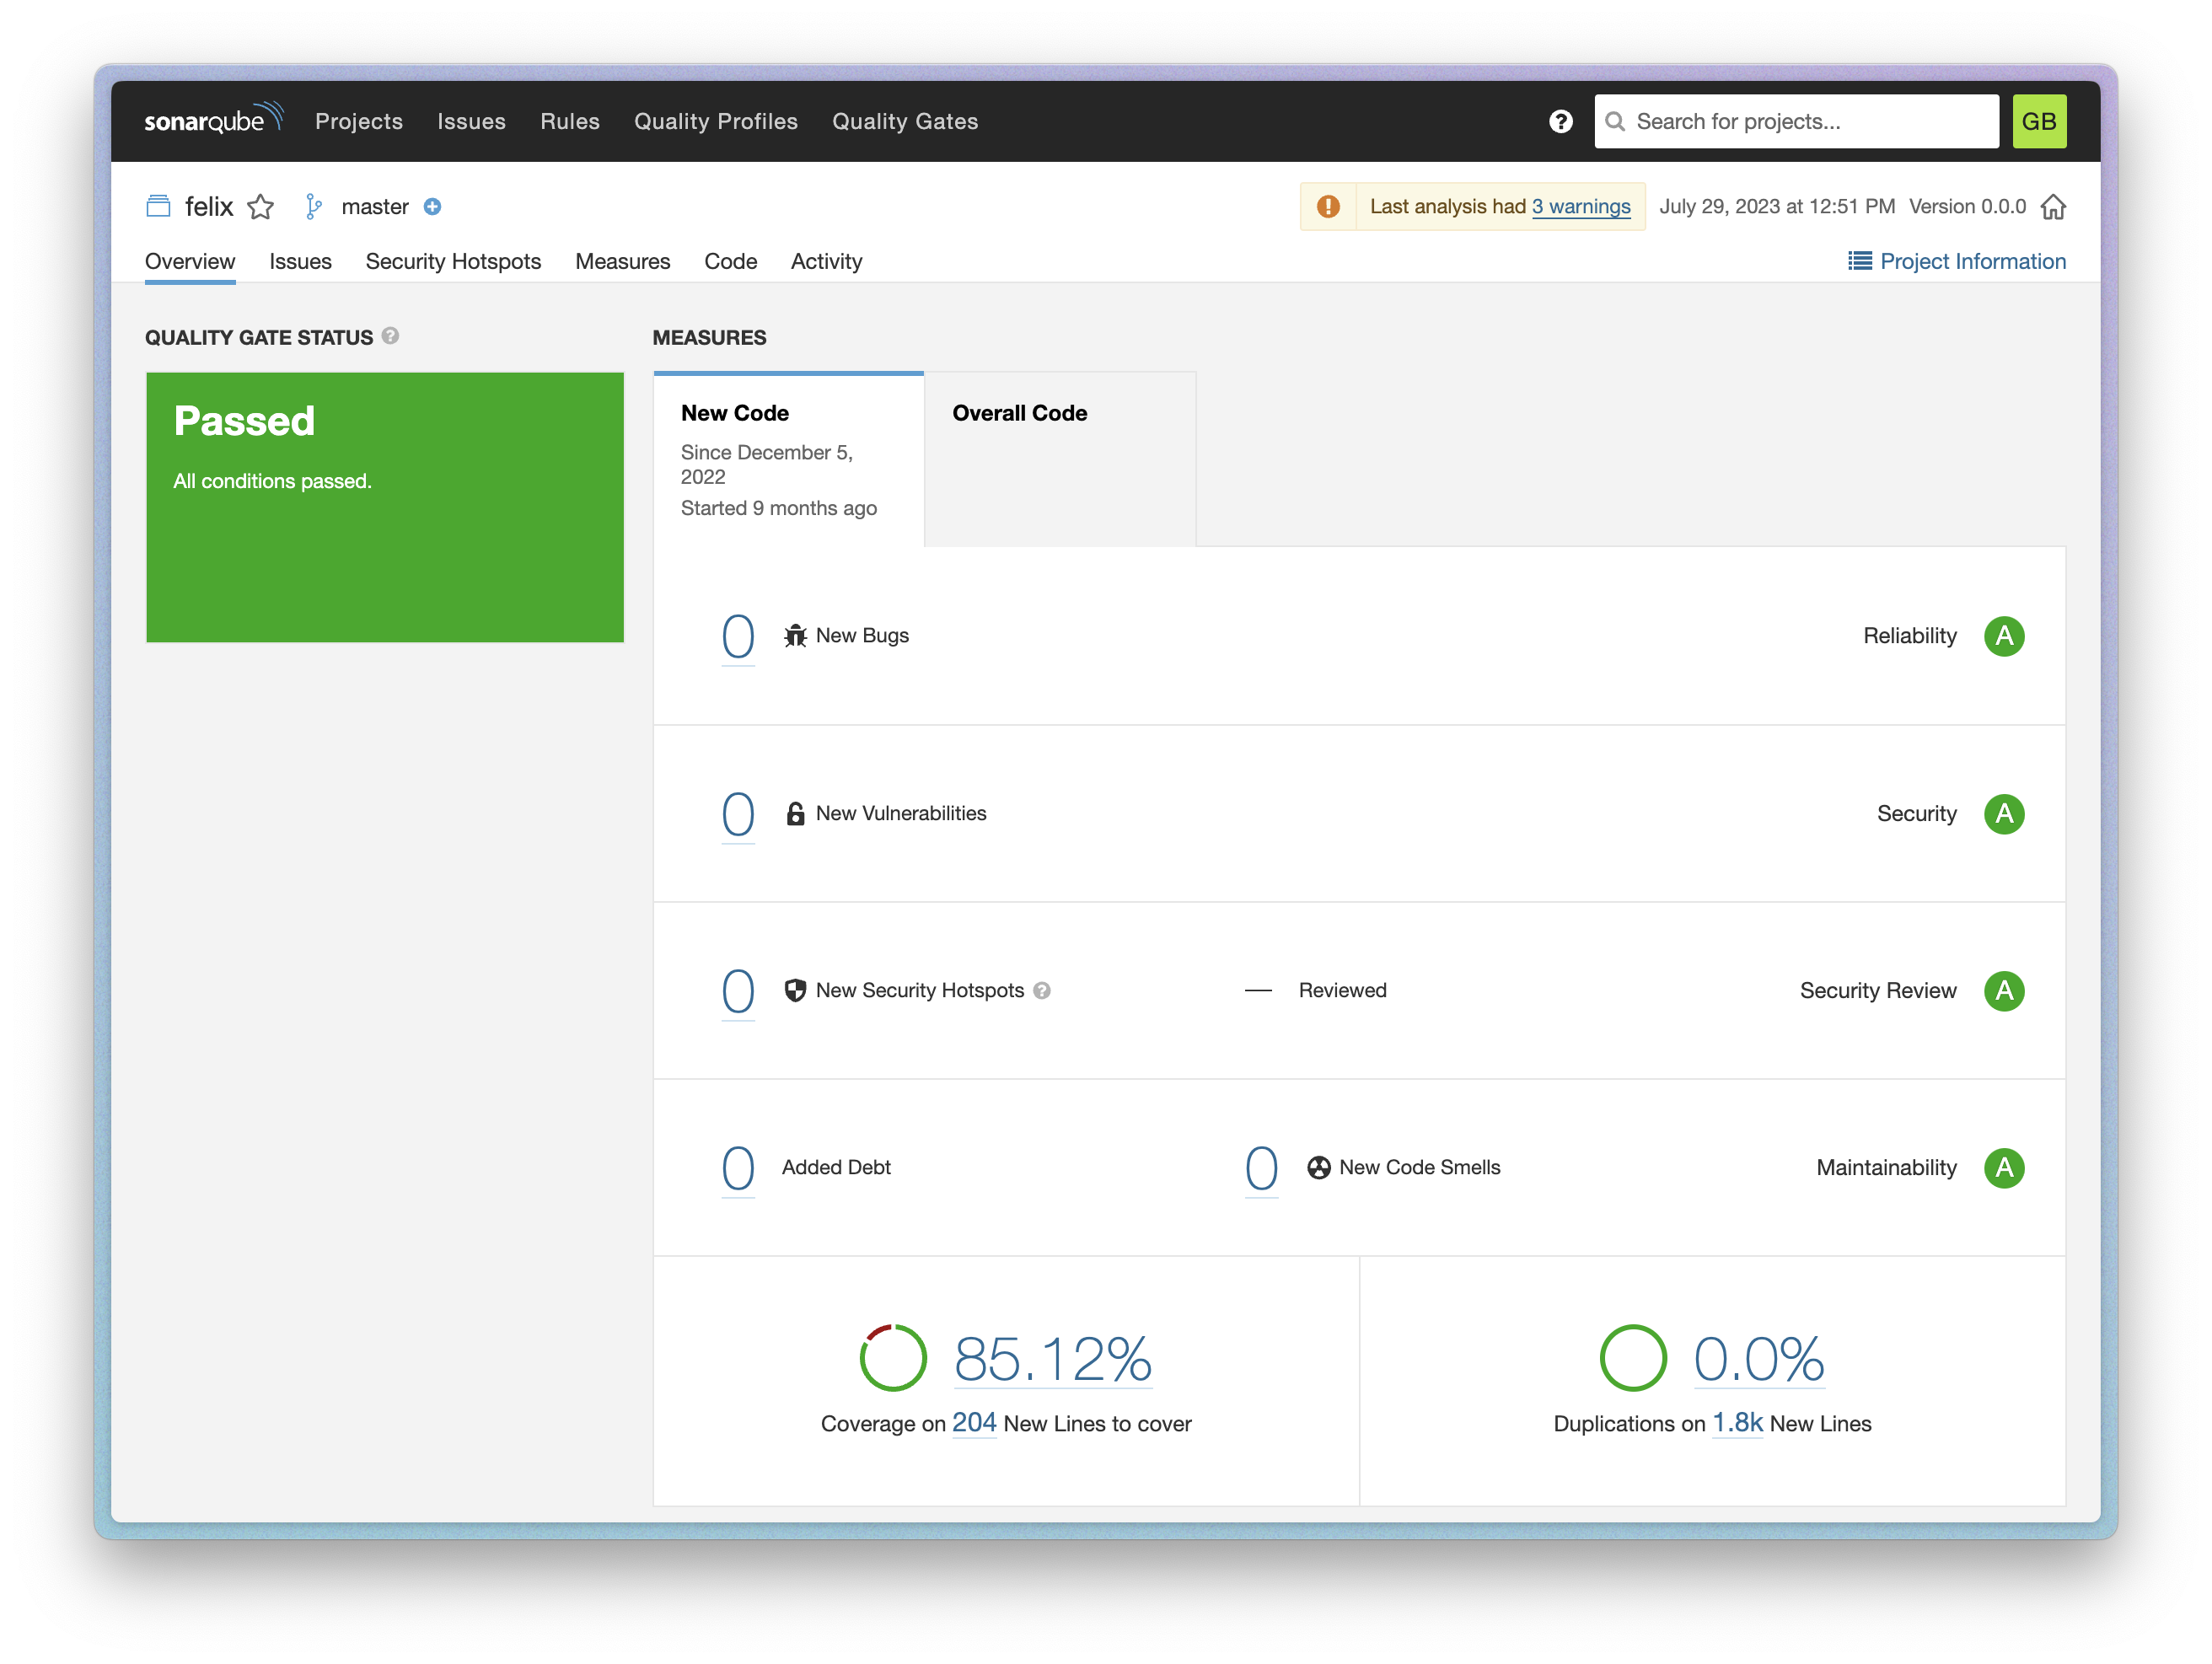
\includegraphics[scale=0.35,center]{screenshots/felix-sonar.png}
      \caption{Logiciel de couverture de tests et d'analyse de code}
  \end{figure}
\textbf{SonarQube} est un outil que nous intégrons dans notre processus
d'intégration continue (CI). Il nous aide à évaluer la qualité de notre
code en identifiant les problèmes potentiels et les opportunités
d'amélioration. Pendant notre CI, SonarQube analyse notre code pour
repérer les bugs, les vulnérabilités et les duplications, tout en
mesurant la couverture des tests.
\newline
\newline
Dans notre approche, nous exigeons qu'au moins \textbf{80\%} du code
soit testé pour que notre pipeline de déploiement puisse fonctionner.
Cette exigence garantit une meilleure stabilité de notre application et
réduit les risques d'erreurs. L'intégration de SonarQube dans notre CI
assure que notre code reste de qualité, sécurisé et conforme aux
meilleures pratiques de développement.
\newline
\newline
La capture d'écran présente les points suivants:
\begin{itemize}
\tightlist
\item
  85.12\% du code de l'application Angular est testé
\item
  Aucun bug n'est présent (erreur dans le code qui provoque un comportement
  indésirable)
\item
  Aucun code smell n'est présent (indicateur suggérant la présence d'un
  problème potentiel dans le code)
\item
  Il n'y a pas de code dupliqué
\item
  Aucun temps de dête technique c'est présent (temps à résoudre les
  divers problèmes cités dans cette liste).
\end{itemize}
\subsection{Contexte de réalisation}
J'ai utilisé les mêmes outils que pour l'acivité 6 pour écrire les tests
unitaires, avec en plus:
\begin{itemize}
\tightlist
\item
  Jest comme framework de tests pour mon application Angular
\item
  Spring Starter Tests pour réaliser les tests sur les microservices
  Angular.
\end{itemize}
Comme montré précédemment j'ai aussi utilisé SonarQube comme logiciel
pour vérifier ma couverture de tests et la qualité du code que j'ai
produit.
\subsection{Conclusion sur l'activité}
Comme pour l'activité 6, peut d'évolutions peuvent avoir lieu, sauf sur le plan technologique, avec des outils toujours plus performants et simple d'utilisations.
\newline
\newline
Cette activité m'a permis d'améliorer ma compréhention des tests et de leur importance sur un projet architécturé en microservices. La prochaine étape est de réaliser des tests End-To-End, pour vérifier que les applications se comportent totalement comme désiré.

\section{Activité 8 - mise en place d’une solution d’intégration continue}
\subsection{Compétence et son fondement}
\textbf{Bloc de compétences}: A5 – Développement d’une solution applicative spécifique et métier selon le projet de développement S.I.
\newline
\textbf{Compétence choisie}: A5C6 –Appliquer l’intégration continue dans le cadre du développement d’une application en utilisant un outil d’intégration continue afin de vérifier la conformité de la solution et les besoins utilisateurs
\newline
\textbf{Détails}: Cette compétence consiste à démonter ma capacité à utiliser un outil d’intégration continu :
\begin{itemize}
  \item installer et paramètre un outil d’intégration continu de mon choix
  \item utiliser les différentes fonctionnalités de l’outil d’intégration choisi
\end{itemize}
\subsection{Présentation et réalisation de l'activité}
\subsubsection{Gitlab CI}
GitLab est une plateforme tout-en-un pour la gestion des projets et du code.
Sa fonctionnalité GitLab CI/CD facilite l'intégration continue et le déploiement automatique.
J'ai opté pour GitLab CI pour l'intégration continue car nous l'utilisons en interne, et sa prise en main, même pour un novice, est relativement simple.
En effet, il s'agit de fichier YAML à écrire, est un format de donnée relativement simple à écrire, à l'aide de tabulations et de données "clefs-valeurs".
\subsubsection{Pipeline d'un microservice du serveur pour l'API REST}
  \begin{figure}[H]
      \centering
      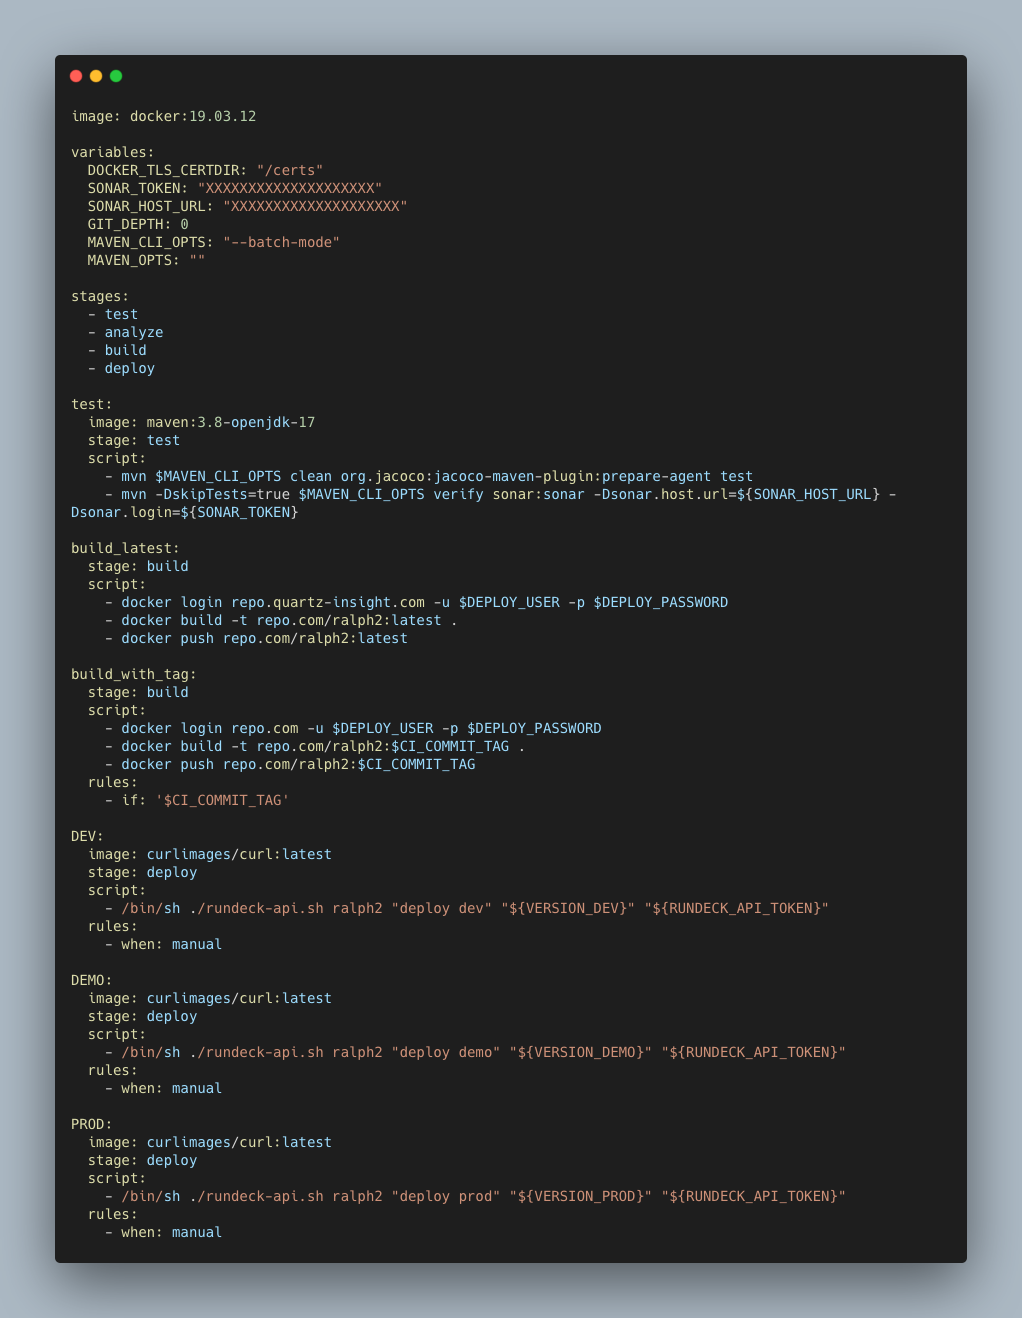
\includegraphics[scale=0.35,center]{screenshots/CICD-ralph.png}
      \caption{Pipeline d'intégration et de déploiement continue d'un microservice d'API REST}
  \end{figure}
  Cette pipeline GitLab suit plusieurs étapes pour tester, construire et
déployer une application :
\begin{enumerate}
\def\labelenumi{\arabic{enumi}.}
\tightlist
\item
  \textbf{Configuration globale} :
  \begin{itemize}
  \tightlist
  \item
    L'image Docker \texttt{docker:19.03.12} est utilisée comme image de
    base.
  \item
    Différentes variables sont définies, comme les informations
    d'authentification Docker, le token SonarQube, l'URL du serveur
    SonarQube, la profondeur du git, et des options Maven.
  \end{itemize}
\item
  \textbf{Stages} :
  \begin{itemize}
  \tightlist
  \item
    Plusieurs étapes sont définies pour la pipeline : \texttt{test},
    \texttt{analyze}, \texttt{build\ latest}, \texttt{build\_with\_tag},
    \texttt{DEV}, \texttt{DEMO}, et \texttt{PROD}.
  \end{itemize}
\item
  \textbf{Étape de test (\texttt{test})} :
  \begin{itemize}
  \tightlist
  \item
    Utilisation de l'image Maven pour exécuter les tests.
  \item
    Nettoyage du projet Maven.
  \item
    Exécution des tests avec JaCoCo pour mesurer la couverture.
  \item
    Exécution de SonarQube pour l'analyse de code statique avec le token
    et l'URL fournis.
  \end{itemize}
\item
  \textbf{Étapes de construction d'images Docker (\texttt{build\ latest}
  et \texttt{build\_with\_tag})} :
  \begin{itemize}
  \tightlist
  \item
    Ces étapes construisent et poussent des images Docker vers un
    registre.
  \item
    L'étape \texttt{build\ latest} construit une image avec l'étiquette
    \texttt{latest}.
  \item
    L'étape \texttt{build\_with\_tag} construit une image avec
    l'étiquette égale au tag du commit.
  \item
    La règle conditionnelle permet à \texttt{build\_with\_tag} de
    s'exécuter uniquement si un tag de commit est présent
    (\texttt{if:\ \textquotesingle{}\$CI\_COMMIT\_TAG\textquotesingle{}}).
  \end{itemize}
\item
  **Étapes de déploiement (\texttt{DEV}, \texttt{DEMO}, \texttt{PROD}) :
  \begin{itemize}
  \tightlist
  \item
    Utilisation d'une image Curl pour effectuer des appels HTTP vers
    Rundeck, notre outil d'automatisation de déploiement (pour mettre à
    jour les images Docker et les déployer sur notre infrastructure).
  \item
    Chaque étape correspond à un environnement de déploiement.
  \item
    Les scripts d'exécution de déploiement sont déclenchés manuellement
    (\texttt{when:\ manual}) et appellent l'API Rundeck pour déclencher
    le déploiement vers chaque environnement avec les versions
    appropriées.
  \end{itemize}
\end{enumerate}
Cette pipeline réalise des tests, construit des images Docker, et
effectue des déploiements vers différents environnements en utilisant
des scripts et des appels d'API spécifiques.
\subsubsection{Pipeline d'un microservice du serveur pour le client web}
  \begin{figure}[H]
      \centering
      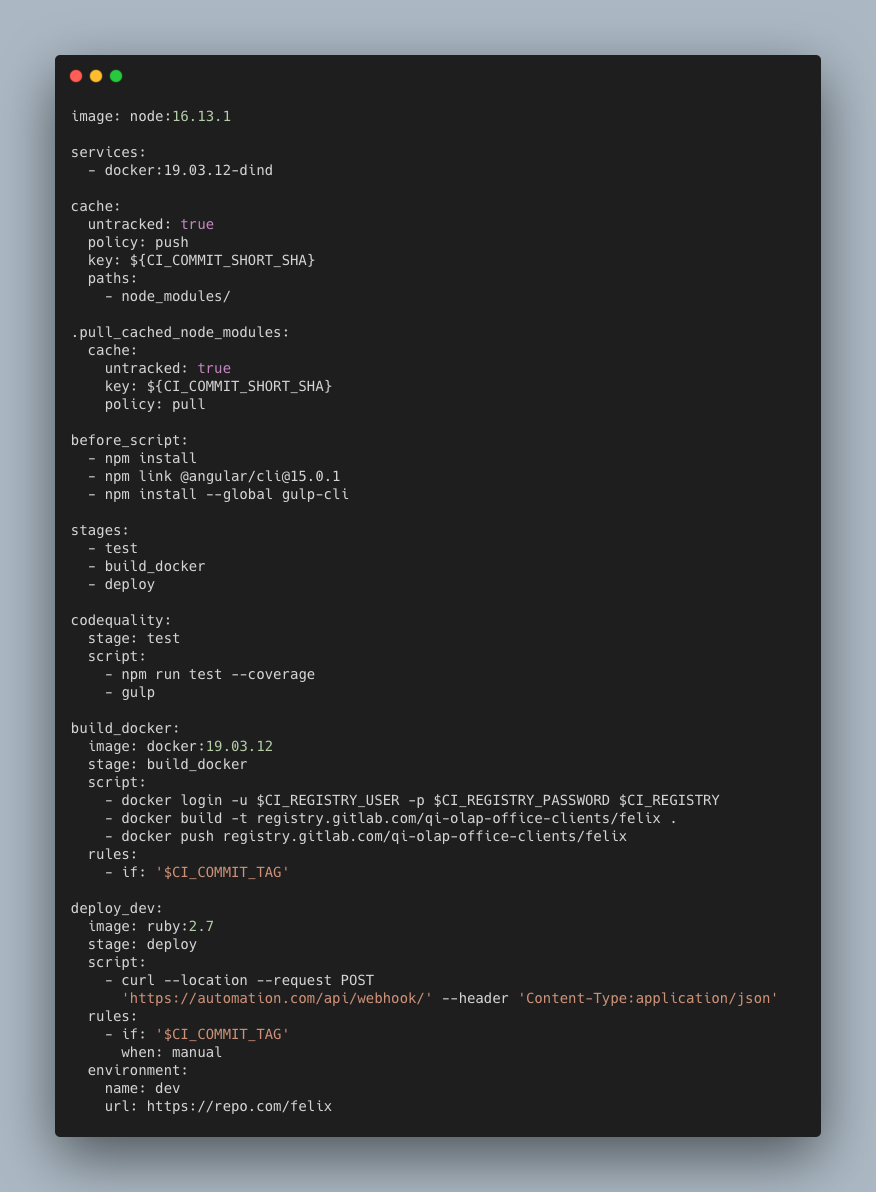
\includegraphics[scale=0.35,center]{screenshots/CICD-Felix.png}
      \caption{Pipeline d'intégration et de déploiement continue du microservice de l'interface web}
  \end{figure}
  Cette pipeline GitLab comporte les étapes suivantes pour la
construction, les tests, la construction d'images Docker et le
déploiement d'une application :

\begin{enumerate}
\def\labelenumi{\arabic{enumi}.}
\tightlist
\item
  \textbf{Configuration de l'image et des services} :

  \begin{itemize}
  \tightlist
  \item
    L'image de base utilisée est \texttt{node:16.13.1}.
  \item
    Les services comprennent Docker (\texttt{docker:19.03.12-dind}),
    pour construire des images Docker dans le pipeline.
  \end{itemize}
\item
  \textbf{Configuration du cache} :

  \begin{itemize}
  \tightlist
  \item
    Le cache est configuré pour des fichiers non suivis
    (\texttt{untracked:\ true}).
  \item
    La politique de cache est définie pour le push et le pull.
  \item
    La clé du cache est basée sur le hachage court du commit
    (\texttt{CI\_COMMIT\_SHORT\_SHA}).
  \item
    Les dossiers \texttt{node\_modules/} et d'autres dépendances sont
    inclus dans le cache.
  \end{itemize}
\item
  \textbf{Étapes du pipeline} :

  \begin{itemize}
  \tightlist
  \item
    \textbf{codequality} (étape de test) :

    \begin{itemize}
    \tightlist
    \item
      L'application est testée et sa couverture est mesurée.
    \end{itemize}
  \item
    \textbf{build\_docker} (étape de construction d'image Docker) :

    \begin{itemize}
    \tightlist
    \item
      Une image Docker est construite à partir du dossier de
      l'application.
    \item
      Authentification Docker est effectuée via les informations du
      registre GitLab.
    \item
      L'image est ensuite poussée vers le registre GitLab.
    \end{itemize}
  \end{itemize}
\item
  \textbf{Règles de déploiement conditionnel} :

  \begin{itemize}
  \tightlist
  \item
    L'étape \textbf{build\_docker} est exécutée seulement si la
    condition \texttt{\$CI\_COMMIT\_TAG} est vraie (lorsqu'un tag est
    ajouté au commit).
  \end{itemize}
\item
  \textbf{Déploiement vers l'environnement de développement (dev)} :

  \begin{itemize}
  \tightlist
  \item
    \textbf{deploy\_dev} (étape de déploiement) :

    \begin{itemize}
    \tightlist
    \item
      Une image Ruby est utilisée pour cette étape.
    \item
      Une requête POST est envoyée à l'URL du webhook pour déclencher le
      déploiement automatisé.
    \item
      Cette étape est déclenchée manuellement (\texttt{when:\ manual}).
    \item
      Les détails de l'environnement de développement sont configurés, y
      compris l'URL de déploiement.
    \end{itemize}
  \end{itemize}
\end{enumerate}

Cette pipeline accomplit des tâches allant de la construction à la
distribution automatisée de l'application, en passant par les tests et
la création d'images Docker, tout en étant flexible grâce à des
conditions et des déclencheurs spécifiques.
\subsection{Contexte de réalisation}
Cette activité, hormis les outils et leurs utilisations, n'a que peu de changement à venir dans son fonctionnement.
Les améliorations disponibles seront une meilleure interface, surement à travers une page web, sans avoir à écrire un fichier au format YAML.
\subsection{Conclusion sur l'activité}
En concluant sur cette activité, j'ai pu utiliser GitLab CI/CD dans un cadre d'intégration continue.
Cette solution a grandement facilité la gestion et l'automatisation de des tâches lors du dévelopement des microservices.
La simplicité d'utilisation de GitLab CI/CD m'a permis de mettre en place les pipelines d'intégration continue, sans difficulté particulière.

\section{Activité 9 - validation fonctionnelle et rédaction de la documentation pour les utilisateurs}
\subsection{Compétence et son fondement}
\textbf{Bloc de compétences}: A5 – Développement d’une solution applicative spécifique et métier selon le projet de développement S.I.
\newline
\textbf{Compétence choisie}: A5C7 – Vérifier la conformité entre la solution développée ou paramétrée et les fonctionnalités attendues à partir des retours des directions métiers afin de rédiger la documentation et les référentiels orientés utilisateurs
\newline
\textbf{Détails}: Cette compétence consiste à démonter ma capacité à rédiger une documentation utilisateur :
\begin{itemize}
  \item comparer la réalisation technique et le cahier des charges
  \item détailler avec une bonne qualité rédactionnelle la documentation utilisateur
\end{itemize}
\subsection{Présentation et réalisation de l'activité}
  J'ai utilisé GitLab pour comparer la réalisation technique avec le
cahier des charges en suivant ces étapes. Tout d'abord, j'ai créé des
``issues'' pour chaque fonctionnalité décrite dans le cahier des
charges. Ensuite, j'ai lié ces issues aux ``merge requests''
correspondants dans lesquels les modifications techniques ont été
apportées. Pendant le processus de développement, j'ai régulièrement mis
à jour les états des issues pour refléter l'avancement. Une fois les
développements terminés, j'ai procédé à des revues de code et de tests
avec les membres de l'équipe pour s'assurer de la conformité de la
réalisation avec les exigences du cahier des charges. Enfin, j'ai
utilisé les fonctionnalités de suivi de GitLab, comme les tableaux
Kanban et les rapports d'avancement, pour visualiser les progrès et
m'assurer que chaque issue était liée à la réalisation technique
correspondante.
  \begin{figure}[H]
      \centering
      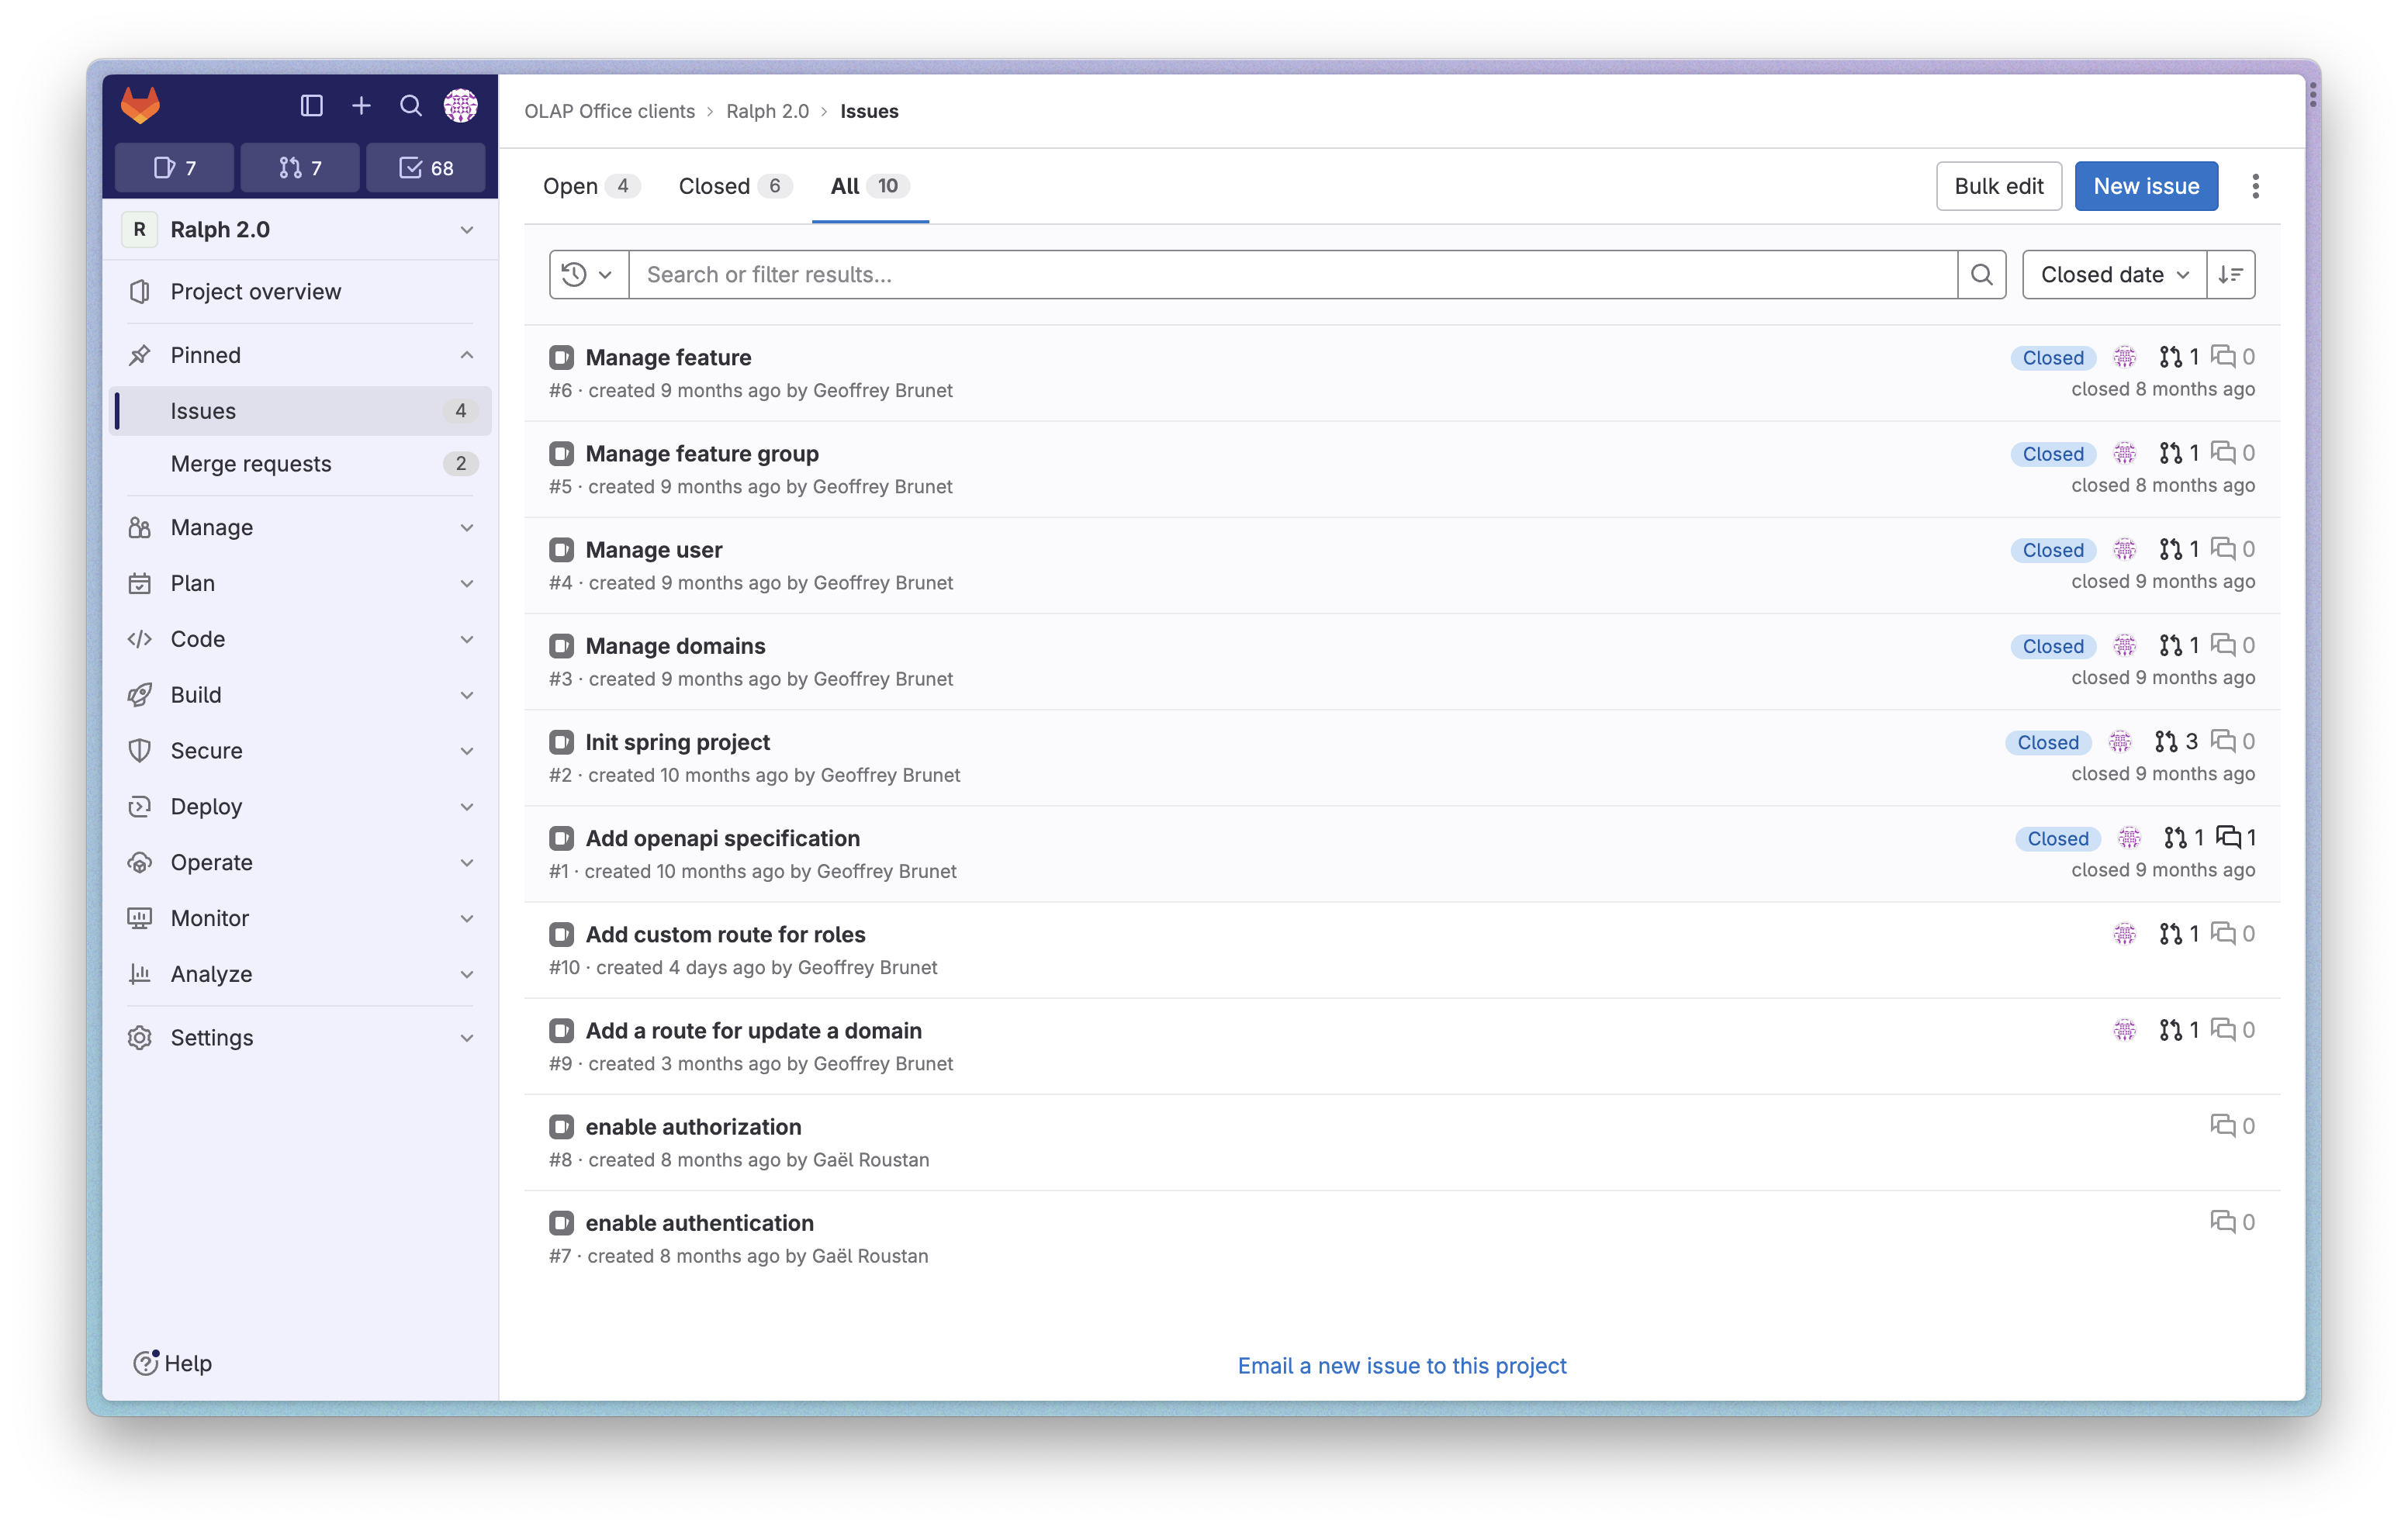
\includegraphics[scale=0.35,center]{screenshots/issues-gitlab.png}
      \caption{Suivi des étapes clefs du développement sur Gitlab}
  \end{figure}
  J'ai utilisé Docusaurus pour créer la documentation utilisateur. J'ai
suivi ces étapes :

\begin{enumerate}
\item
  \textbf{Installation et Configuration} : J'ai installé Docusaurus et
  configuré le projet.
\item
  \textbf{Organisation du Contenu} : J'ai structuré la documentation en
  sections basées sur les fonctionnalités, et les APIs.
\item
  \textbf{Rédaction en Markdown} : J'ai rédigé le contenu dans les fichiers
  Markdown Extended, en incluant des images et des liens.
\item
  \textbf{Validation Utilisateur} : J'ai sollicité les retours des
  membres du pôle R&D pour m'assurer de la clarté et de l'utilité du contenu.
\item
  \textbf{Publication en Ligne} : J'ai publié la documentation en ligne
  pour offrir un accès facile aux utilisateurs.
\end{enumerate}
J'ai utilisé docusaurus qui permet la création d'une documentation
simplement et accessible pour les utilisateurs.
  \begin{figure}[H]
      \centering
      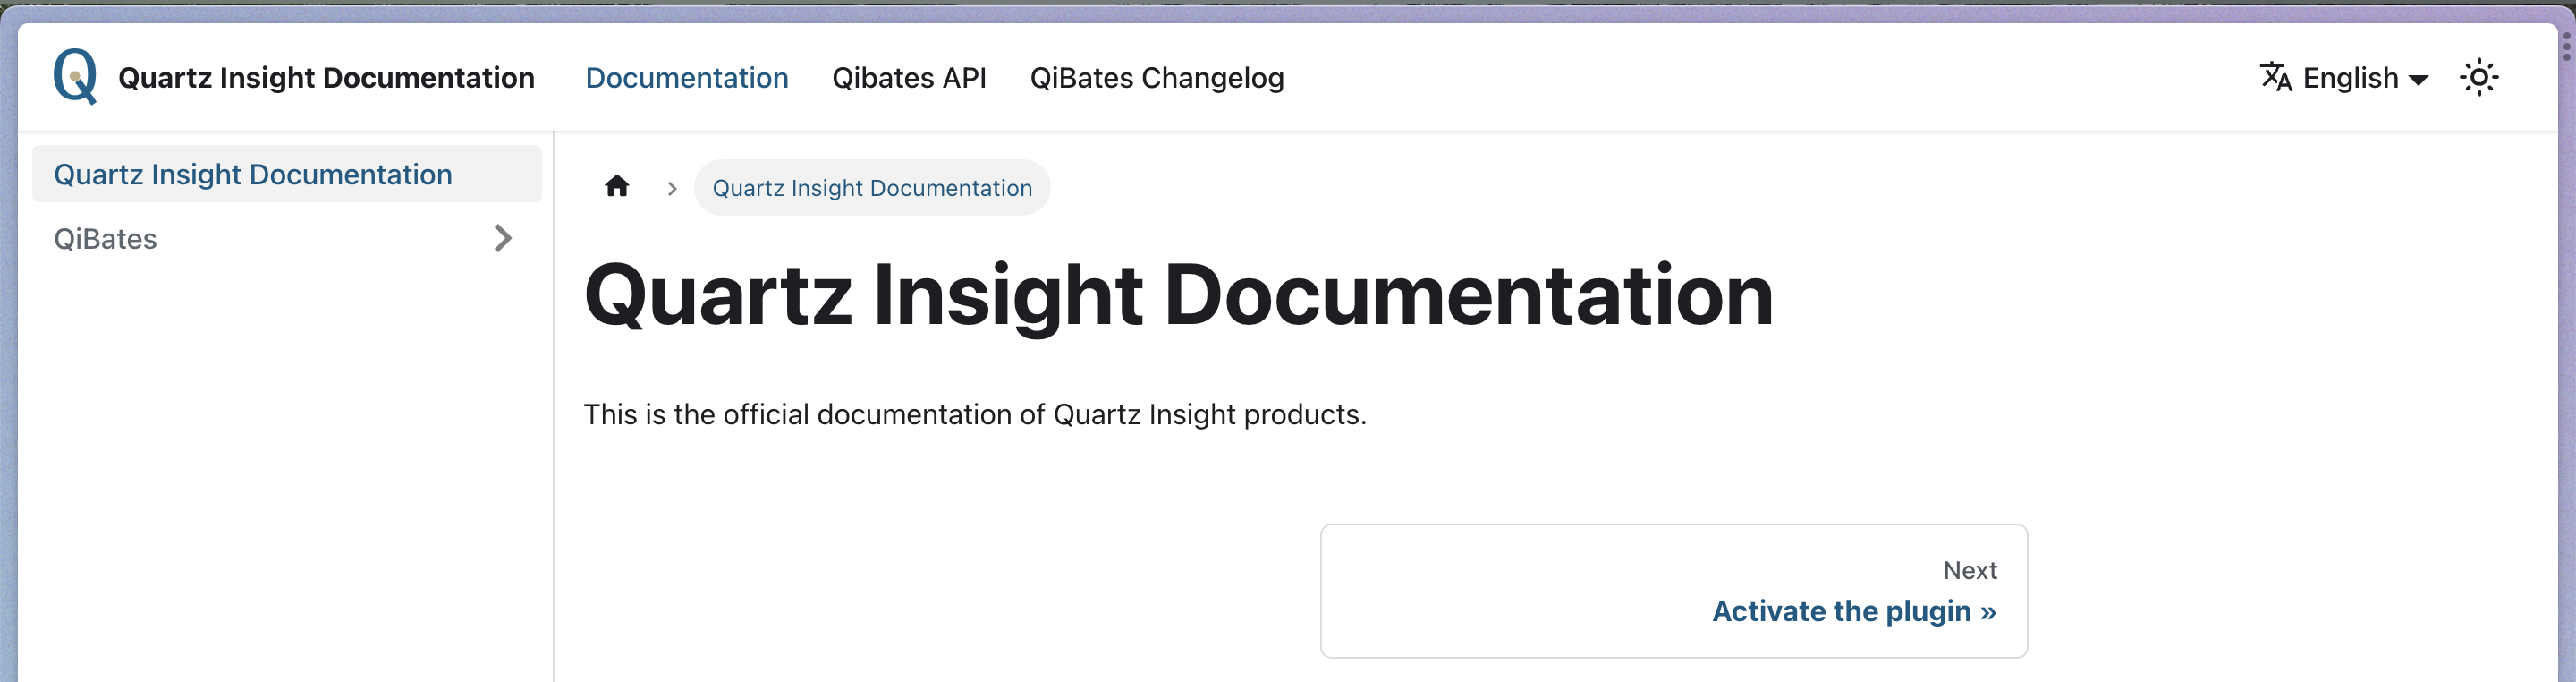
\includegraphics[scale=0.30,center]{screenshots/documentation.png}
      \caption{Documentation utilisateur en ligne}
  \end{figure}
\subsection{Contexte de réalisation}
J'ai donc utilisé Gitlab pour la gestion et le suivi de projet, et j'ai utilisé
Docusaurus pour réaliser la documentation utilisateur et des APIs. Ces deux technologies
sont open-source, et pour Gitlab nous utilisons la version hebergée mais gratuite.
\subsection{Conclusion sur l'activité}
La compétence liée à la validation fonctionnelle et à la rédaction de la
documentation a évolué ces dix dernières années en raison de
l'apparition de nouveaux outils de documentation et de collaboration en
ligne.
\newline
\newline
J'ai acquis des compétences en comparant la réalisation technique avec
le cahier des charges grâce à l'utilisation de GitLab pour suivre les
changements et les commentaires, sans rencontrer de grande difficulté,
et en ayant été force de proposition pour l'utilisation de Docusaurus.

\section{Activité 10 - formation des utilisateurs, mise en place d’une enquête de satisfaction ultérieure}
\subsection{Compétence et son fondement}
\textbf{Bloc de compétences}: A5 – Développement d’une solution applicative spécifique et métier selon le projet de développement S.I.
\textbf{Compétence choisie}: A5C8 - Conduire le changement auprès des métiers lors du déploiement d’une solution applicative ou intégrée en mettant en place une démarche de participation, de communication et de formation pour accompagner les utilisateurs à l’intégration du nouvel outil dans leurs habitudes de travail
\newline
\textbf{Détails}: Cette compétence consiste à démonter ma capacité à proposer un plan d’action de conduite de changement :
\begin{itemize}
  \item identifier les actions à mener sur les 4 axes (Informer, communiquer, former, faire participer) :
  \item présenter différents outils de changement (FutureWheel, Modèle transactionnel de William Bridge,...)
  \item mettre en application son plan de conduite de changement via un outil
\end{itemize}
\subsection{Présentation et réalisation de l'activité}
\subsubsection{Actions sur 4 axes}
Pour réussir la conduite du changement dans mon projet, j'ai mis en
place des actions spécifiques sur les quatre axes clés :
\begin{enumerate}
\def\labelenumi{\arabic{enumi}.}
\item
  \textbf{Informer} : J'ai élaboré des communications claires et
  concises pour informer les utilisateurs (actuellement les membres du
  pôle R\&D) des raisons du changement, de ses avantages et des étapes à
  venir. J'ai utilisé des emails, des messages sur Microsoft Teams et
  des réunions pour diffuser ces informations.
\item
  \textbf{Communiquer} : J'ai créé une communication continue en mettant
  en place des canaux de discussion tels que des groupes de discussion
  en ligne ou des sessions de questions-réponses, toujours avec
  Microsoft Teams.
\item
  \textbf{Former} : J'ai organisé des sessions de formation adaptées aux
  besoins des utilisateurs. Ces sessions ont couvert les fonctionnalités
  clés de la nouvelle solution, avec des démonstrations pratiques et des
  exercices. Cela a renforcé leur compréhension et leur confiance dans
  l'utilisation du nouvel outil.
\item
  \textbf{Faire Participer} : J'ai encouragé la participation active des
  utilisateurs tout au long du processus. J'ai sollicité leurs
  commentaires lors des phases de test, en tenant compte de leurs
  suggestions pour améliorer l'expérience utilisateur. Leur implication
  a contribué à créer un sentiment d'appartenance au projet.
\end{enumerate}
\subsubsection{Présentation des outils de changement}
Lors de la conduite du changement, j'ai exploré divers outils pour
faciliter la transition en douceur vers la nouvelle solution. Deux de
ces outils sont :
\begin{enumerate}
\def\labelenumi{\arabic{enumi}.}
\item
  \textbf{FutureWheel} : Le FutureWheel est un modèle visuel qui permet
  aux individus et aux équipes de visualiser leurs objectifs futurs.
  J'ai utilisé cet outil pour aider les utilisateurs à envisager les
  avantages et les opportunités que la nouvelle solution apporterait à
  leurs activités quotidiennes. Cela a permis de créer un sentiment
  positif et d'anticiper les résultats positifs du changement.
\item
  \textbf{Modèle transactionnel de William Bridge} : Ce modèle propose
  une approche pour gérer les émotions et les résistances liées au
  changement. J'ai appliqué ce modèle pour aider les utilisateurs à
  passer par les différentes étapes émotionnelles du changement, telles
  que la phase de deuil pour ce qui est laissé derrière, la phase de
  transition où ils se familiarisent avec le nouveau, et enfin la phase
  d'acceptation.
\end{enumerate}
\subsubsection{Application d'un plan de conduite de changement}
Dans mon projet, j'ai mis en pratique le Modèle transactionnel de
William Bridge en organisant des sessions de sensibilisation et de
discussions avec les membres du pôle R\&D. J'ai identifié leurs
préoccupations, leurs résistances et leurs émotions vis-à-vis du
changement. Ensuite, j'ai adapté ma communication en fonction de ces
étapes émotionnelles, en fournissant des informations rassurantes et en
expliquant les bénéfices concrets de la nouvelle solution. J'ai
également encouragé la participation active des utilisateurs en leur
offrant des opportunités de poser des questions, de partager leurs idées
et de contribuer au processus. En utilisant ce modèle, j'ai pu aider les
membres de l'équipe à surmonter leurs appréhensions et à embrasser le
changement de manière plus positive et constructive.
\subsection{Contexte de réalisation}
J'ai réalisé ce plan avec les collaborateurs avec des communications
synchrones (réunions en visioconférence) et asynchrones (par messages et
emails), étant en télétravail la totalité du temps. Les outils utilisés
sont donc Microsoft Teams et Outlook, ainsi que le modèle transactionnel
de William Bridge comme cité précédemment.
\subsection{Conclusion sur l'activité}
Au cours des dernières années, la conduite du changement a évolué en
raison des avancées technologiques et des nouvelles réglementations. Les
évolutions à venir pourraient inclure une plus grande utilisation des
plateformes en ligne pour la communication et la formation, ainsi qu'une
adaptation aux méthodes de travail à distance.
\newline
\newline
Pour mettre en place le plan de conduite de changement, je me suis aidé
des compétences acquises en formation et des ressources fournies par les
formateurs.

\chapter{Informations complémentaires}
\section{Gestion de projet}
J'ai choisi d'adopter une approche de gestion de projet agile pour
réaliser mon projet. J'ai opté pour la méthodologie Scrum, avec des
itérations de 2 semaines appelées ``sprints''.
\newline
Lors de la planification de chaque sprint, j'ai utilisé la technique du
poker planning pour estimer la complexité des tâches et des problèmes à
résoudre. Cette méthode collaborative a impliqué tous les membres de
l'équipe dans la définition des difficultés et des délais, me permettant
d'avoir un avis extérieur sur la difficulté possible des tâches du
projet.
\newline
Les réunions matinales quotidiennes ont favorisé la communication et la
résolution rapide des problèmes rencontrés. Ces réunions étaient
essentielles pour permettre aux équipes de connaître l'avancé du projet.
\newline
En fin de sprint, j'ai effectué une rétrospective pour évaluer ce qui a
bien fonctionné et ce qui pourrait être amélioré. Cette approche
itérative m'a permis d'adapter le projet en cours de route et de
répondre aux changements.
\section{Gestion des coûts}
En tant qu'alternant, j'ai pris en compte la gestion des coûts pour mon
projet. Les principaux éléments de coûts comprenaient mon salaire en
tant qu'alternant, ainsi que les ressources informatiques nécessaires
pour le développement. J'ai utilisé des machines virtuelles et des
systèmes de gestion de base de données (SGBD) hébergés sur le cloud
d'Orange pour déployer et tester mon application. Ces services cloud ont
engendré des coûts liés à leur utilisation. J'ai veillé à surveiller et
à optimiser ces coûts tout au long du projet en utilisant des outils de
suivi et en ajustant les ressources selon les besoins. Cette approche
m'a permis de maintenir le projet dans les limites budgétaires définies
tout en garantissant la continuité et la qualité du développement.
\newline
\newline
Les coûts ont donc été divisés en deux catégories:
\begin{itemize}
\tightlist
\item
  mon salaire en tant qu'alternant
\item
  le coût de ma formation à l'EPSI et des formations en interne (comme
  sur Angular par exemple)
\item
  le coût de l'infrastructure sur le cloud Orange.
\end{itemize}

\chapter{Conclusion}

\section{Résumé}
Ce projet m'a permis d'acquérir une expérience précieuse dans le dévelop\-pement de microservices, en utilisant une combinaison de technologies telles que PostgreSQL, Spring Boot et Angular.
La réalisation de ce projet m'a permis de mettre en pratique mes connaissances théoriques acquises au cours de mes études.
J'ai dû faire face à des défis techniques, tels que la modélisation de la base de données et la mise en œuvre des fonctionnalités clés de l'application.
Ce projet m'a également sensibilisé à l'importance de la planification, de la gestion du temps et de la communication efficace dans un contexte professionnel.
J'ai appris à hiérarchiser les tâches, à gérer les priorités et à respecter les délais, tout en maintenant une communication régulière avec mon équipe et en fournissant des mises à jour régulières sur l'avancement du projet.
\newline
\newline
En conclusion, ce projet de gestion des licences utilisateurs chez Quartz-Insight a été une expérience enrichissante qui m'a permis de consolider mes compétences en développement de microservices et en gestion de projet de bout-en-bout pour un logiciel.
Je suis fier d'avoir réussi à réaliser un produit fonctionnel et utile pour les entreprises, tout en respectant les exigences et les contraintes du projet.
Je suis reconnaissant envers l'équipe de Quartz-Insight pour leur soutien et leur expertise tout au long du projet.
\newline
\newline
Le code de mon dossier professionnel peut être trouvé à l'adresse suivante: \href{https://github.com/GeoffreyBrunet/memoire-i2}{https://github.com/GeoffreyBrunet/memoire-i2}.

\section{Ouverture sur l'avenir}

\subsection{L'entreprise et ses perspectives}
Grâce à son expertise approfondie dans le domaine de la BI et de l'EPM, l’entreprise se distingue par sa capacité à proposer des stratégies de gestion efficaces, des modélisations de données précises et des analyses approfondies pour aider les entreprises à prendre des décisions éclairées.
Son équipe de consultants hautement qualifiés travaille en étroite collaboration avec les clients pour comprendre leurs besoins spécifiques et résoudre leurs problèmes, voir être pro-actifs par rapport à ceux-ci.
\newline
\newline
Les perspectives de Quartz-Insight en tant que PME sont prometteuses.
Avec son approche personnalisée, son agilité et son engagement continu envers l'innovation, l'entreprise est bien positionnée pour étendre sa clientèle et se démarquer sur le marché de la BI et de l'EPM.
La taille réduite de l'entreprise lui permet également de maintenir une culture d'entreprise forte et un haut niveau de service client, ce qui contribue à sa réputation positive.

\subsection{Le service et ses évolutions}
Grâce à la vente de licences en constante augmentation, auprès d’une clientèle de plus en plus variée, la pérennité du service est assurée. Mais de nouvelles contraintes et nouvelles améliorations peuvent être mises en place:
\begin{enumerate}
  \item \textbf{Ajout de nouveaux connecteurs et intégration de nouvelles sources de données}:
    \ En permettant l'intégration de nouvelles sources de données, telles que des bases de données supplémentaires, des services cloud ou des API externes, les utilisateurs auront une plus grande flexibilité dans l'exploration de diverses sources.
  \item \textbf{Amélioration de la supervision}:
    \ En intégrant des fonctionnalités de supervision avancées, telles que des tableaux de bord de surveillance en temps réel, des alertes automatisées en cas d'anomalies ou de dépassement de seuils, et des rapports de performance détaillés, les administrateurs et responsables pourront superviser efficacement les performances et l'utilisation de Qibates.
    \ Cela facilitera la détection précoce des problèmes, l'optimisation des ressources et la prise de décisions basées sur des données précises.
  \item \textbf{Élaboration d'un Plan de Reprise d'Activité (PRA)}:
    \ Pour assurer la continuité des opérations en cas d'incident majeur ou de catastrophe, il est essentiel de développer un PRA solide pour Qibates.
    \ Ce plan devrait inclure des procédures détaillées pour la sauvegarde régulière des données, la restauration du système, la reprise des opérations critiques, la communication avec les parties prenantes, ainsi que des tests réguliers pour s'assurer de l'efficacité du plan.
    \ Un PRA bien élaboré garantira une reprise rapide et efficace des activités en cas d'urgence, minimisant ainsi l'impact sur les utilisateurs et l'entreprise dans son ensemble.
  \item \textbf{Amélioration de la documentation}:
    \ En fournissant une documentation détaillée et des ressources de support, la prise en main de Qibates par les utilisateurs seras facilitée.
\end{enumerate}

\subsection{Les apports professionnels et personnels}
Ce projet réalisé au sein de Quartz-Insight lors de mon alternance a été une expérience professionnelle et personnelle enrichissante.
Sur le plan professionnel, j'ai pu mettre en pratique mes compétences techniques en développement de microservices, en utilisant des technologies telles que PostgreSQL, Spring Boot et Angular.
J'ai renforcé ma compréhension des processus de développement logiciel et des bonnes pratiques. 
Travailler en équipe m'a permis d'améliorer ma communication et ma collaboration.
Sur le plan personnel, j'ai gagné en confiance en moi grâce aux succès obtenus et j'ai développé mon autonomie en prenant des initiatives et en résolvant des problèmes de manière indépendante.
En résumé, ce projet m'a apporté des compétences techniques solides, renforcé ma confiance en moi, développé mon autonomie et élargi mon réseau professionnel, ce qui constituera des atouts précieux pour ma future carrière en tant qu'ingénieur logiciel.

\subsection{Avenir professionnel}
Pour mon avenir professionnel, je suis passionné par l'optimisation des performances en tant qu'ingénieur en logiciel. Je suis attiré par le développ\-ement frontend avec des langages et libraries tels que TypeScript, React ou Svelte, ainsi que le développement backend avec Rust. Mon objectif est de créer des applications web rapides et performantes en réduisant les temps de réponse et en optimisant les requêtes.
J'explore également l'utilisation de Rust compilé en WebAssembly pour exécuter du code hautement performant dans les navigateurs web. Cela me permet de développer des applications web puissantes et réactives, offrant une expérience utilisateur améliorée.
En résumé, mon ambition est de contribuer à des projets stimulants axés sur l'amélioration des performances. Je souhaite devenir un ingénieur en logiciel polyvalent, capable de créer des solutions performantes en utilisant React ou Svelte, TypeScript, Rust et WebAssembly, afin de garantir des expériences utilisateur exceptionnelles et d'optimiser l'efficacité des systèmes.

\appendix
\chapter*{Annexes}

\section*{1. Définition d'EPM (Entreprise Performance Management)}
Processus de gestion qui intègre la planification stratégique, la budgétisation, la prévision et la gestion des performances d'une entreprise pour atteindre ses objectifs.

\section*{2. Définition de BI (Business Intelligence)}
Processus de collecte, d'analyse et de présentation d'informations pertinentes pour prendre des décisions éclairées dans une entreprise.

\section*{3. Définition d'API REST}
Interface qui permet aux applications informatiques de communiquer entre elles via des requêtes HTTP en suivant les principes de l'architecture REST.

\section*{4. Définition de Service monolithique}
Application logicielle regroupant toutes ses fonctionnalités en un seul bloc, sans division en composants distincts.

\section*{5. Définition de Microservices}
Architecture logicielle où une application est décomposée en petits services indépendants, chacun exécutant une fonction spécifique.

\section*{6. Définition de Framework}
Ensemble de composants et de conventions prédéfinis facilitant le développement d'applications en fournissant une structure et des fonctionnalités réutilisables.

\section*{7. Définition de SGBD}
Logiciel permettant de stocker, organiser et manipuler des données de manière structurée.

\section*{8. Définition d'ASP.NET}
Framework de développement web de Microsoft permettant de créer des applications web dynamiques et interactives.

\section*{9. Définition d'Angular}
Plateforme de développement front-end open-source développée par Google, permettant de créer des applications web interactives et réactives.

\section*{10. Définition de Spring Boot}
Framework open-source basé sur Java qui facilite le développement rapide et la création d'applications Java autonomes, en simplifiant la configuration et la gestion des composants.

\section*{11. Définition de PostgreSQL}
Système de gestion de base de données open-source puissant et performant, basé sur le modèle relationnel, capable de gérer de grandes quantités de données et offrant une large gamme de fonctionnalités avancées.

\section*{12. Définition d'ORM (Object-Relational Mapping)}
Technique de programmation qui permet de faire correspondre les objets d'une application avec les enregistrements d'une base de données relationnelle de manière transparente.

\end{document}
